% -*- LaTeX -*-

\part{User's guide}

\chapter{Installation of \vamps}
Because \vamps\ runs on several quite different platforms installation
requires some things to be set. \vamps\ is distributed as source code
only or as source code plus binaries. As I only have access to MS-DOS,
Linux, Sun-OS and OS/2 systems these are the only binaries I can make.

In the case of a {\sc unix} system installation from source
code the following steps are required:
\begin{enumerate}
\item First read the files \fname{0readme} and \fname{0install}.

\item 
Run the \fname{configure} script in the \dirname{src} directory. If you
don't want to install \vamps\ in \dirname{/usr/local} make sure to run
the \fname{configure} script with the
\fname{--prefix=/your/installdir} option. If you have the agl or
\slang\ library installed in a non-standard place set the LDFLAGS
environment variable so that \fname{configure} can find them
(e.g. \fname{setenv LDFLAGS -L/home/schj/lib}). If you don't have
\slang\ now would be a good time to install it.

\item Check the top part of the Makefile in the {\sc src} directory

\item Run make lib, make all and make install.
\end{enumerate}

In case of an MS-DOS system (it should be a 386Sx at least) it is
sufficient to copy all the .exe files to a directory in your
search-path. You should also copy the default {\tt \Index{vamps.rc}}
and {\tt \Index{vamps.sl}} files -- all located in the sllib directory
-- to a place where \vamps\ can find them (set the {\tt \Index{HOME}}
or {\tt VAMPSLIB} environment variable to the directory in which these
files reside).

You will need to have the \slang{} library installed if you want to
compile the program from source. The \slang\ library can be found at
{\tt ftp://space.mit.edu/pub/davis/slang}.

%---------------------------------------------------------------------
\chapter{Program organization}

\section{Introduction}
The main module of \vamps\ is the \vamps\ program itself. It uses a
series of equations to describe the flow of water through a forested
ecosystem.  Preparing input for the \vamps\ program takes quite a
while and is by no means a trivial task. Some 'basic' understanding of
the functioning of forested ecosystems is needed.

REWRITE THIS !!!

To facilitate the data pre- and post-processing some tools are
included: The {\bf \Index{wrini}}(1) program can be used to create
input files at a basic level.  It is mostly used in scripts. The {\bf
\Index{issec}}(1) and {\bf \Index{getstr}}(1) programs can be used to
extract part of output files. For general post-processing however, the
{\bf \Index{vsel}}(1) program is recommend.  This program can produce
data the can be fed directly to plotting programs such as {\bf
\Index{gnuplot}}(1) and {\bf \Index{graph}}(1). {\bf vsel} output can
also be imported into popular spreadsheet programs.
\footnote{Using \slang{} it should be fairly easy to write custom
postprocess-functions. For example the following command gets the
variable {\tt volact} from an output file for all timesteps and
write a two column ascii file that can be read into spreadsheet
software: {\tt mwrite(getts("volact","vamps\_output\_file",-1),"columnfile");}
}

\vamps{} can crash in certain situations. This can have three reasons: {\em
(1)} I have made an error, causing you to discover a genuine bug, (2)
the situation you want to model is beyond the capabilities of \vamps{},
{\em (3)} the timestep estimate done by \vamps{} is not right. The
method that is used to solve Richards equation is rather stable but can
go bezerk given the right combination of boundary conditions and soil
parameters. A lot of precipitation on a {\em very} clayey soil is a
recipe for disaster.  There are some options you can use to circumvent
some problems. They are described in section~\ref{sec:troubles}


\section{System requirements}

If you are not in a hurry a 386Sx MS-DOS based computer with a 1.44Mb
floppy drive is the minimum you need for running \vamps. As most
calculations are done with floating point numbers, a 387 co-processor
will speed up things a lot\footnote{Dramatically might be a better word
as I found out myself}. Djgpp\footnote{A MS-DOS port of the GNU C/C++
compiler which I used to create the .EXE files.} compiled programs
require a {\sc \Index{dpmi}} server\footnote{A freeware {\sc dpmi}
server is included in the distribution. Note that a windows or OS/2
MS-DOS box can also provide {\sc dpmi} service.} and should run with 512
Kb of memory, although 1Mb should be considered a minimum. You need
some disk space as well. The \vamps\ binary does not use a lot of it,
but your input (and certainly output) data will probably by the
biggest users of disk space. \vamps\ is known to run with several
\Index{operating systems}: MS-DOS, Linux, Net-BSD, Sun-OS, AIX 3.2 and OS/2
Warp. 

\section{Defaults file}
%I:DEFAULTS
REWRITE!! Several layers!

Some settings which you want to use in several sessions can be added
to the \vamps\ defaults file. The name of this file is {\tt .vampsrc} on
unix systems or {\tt vamps.rc} or FAT based (MS-DOS or OS/2) systems.
\vamps\ first searches for this file in the current directory, if
this fails the directory to which the HOME environment variable is set
is searched.  After this the directory to which the VAMPSLIB
environment variable is set is searched. If this also fails the
compiled-in {\tt vampslib} directory is searched.  If no defaults file
is found compiled-in defaults will be used. The syntax of the defaults
file is the same as the general input file. Allowed sections and
variables are described in section~\ref{section:defaults} on
page~\pageref{section:defaults}.

If \vamps\ is compiled with \slang\ support it also needs to load
several \slang\ files at startup. These must be present in the
VAMPSLIB directory. If (this is an MS-DOS example) you have installed
\vamps\ in c:\verb-\-vamps you should use the following command to let
\vamps\ find it's files:
\begin{quote}
{\tt set VAMPSLIB=c:\verb-\-vamps}
\end{quote}
In {\sc unix} the command to set an environment variable differs
per shell used, in the c-shell you could use: 
\begin{quote}
{\tt setenv VAMPSLIB /home/usr-x/lib/vamps}
\end{quote}
%E:

\section{Time series and time steps}\label{sec:tstep}
Time series are values of certain variables over time that \vamps\
uses as input. An example of a time series is precipitation.  All time
series \footnote{Time series files must contain two columns, time and
value. Lines starting with \# are regarded as comments (see {\bf
ts(5))}.}  must be listed in the ts section of the input file.

The precipitation time series is quite special because it {\em must} be
present. This is because this time series determines the time steps
that \vamps\ make with it's x-column. This column should be in days or
fractions of day (i.e. 1.5 is halfway day 1). Time steps may vary
within one run. The following example of a precipitation input file
shows how this is done:
\begin{verbatim}
# This is a comment
# Precipitation from the no-name site 
# time in days         amounts in cm/day (intensity!)
0.5		0.6
1.0		0.9
2.0		0.7
2.1		0.9
2.2		0.7
2.3		0.5
3.0		0.8
3.5		0.0
\end{verbatim}
In this case 0.9 cm/day fell between day 2.0 and day 2.1 amounting to
$ 0.9  (2.1 - 2.0 = 0.09)$ cm.  There are
several things that must be remembered with respect to time-steps and
input-files in \vamps{}:
\begin{enumerate}
\item Units are in cm/day. With precipitation you might have to convert
your data to intensities.
\item The time in the x-column is the {\em end} of an interval. In
of the above example output given at time 3.0 is calculated from the
situation at time 2.3 after including the precipitation
from time 3.0.  The duration of this time-step is 0.7 days (3.0 - 2.3). This
implies that in the case of the first record no duration of the time-step is
known. \vamps\ defaults to one day for the first time-step. You can change
this using the \inivar{firststep} variable in the \inisec{time} section of the
input file.
\item At present the x-column in all files but the precipitation-file
is ignored (that is, it must be present, but \vamps\ does not check
the time-values).
\end{enumerate}


\section{The principle of layers in the soil section}\label{sec:physlay}
The \inivar{layers} variable in the \inisec{soil} section determines the
number of layers used by \vamps\ in the {\em calculations}
\footnote{Actually {\bf nodes} would be a better name for this
variable}. The number of {\em physical} layers (with different
$K_{sat}$ for example) is determined by the number of \inisec{layer\_n}
sections you have. Figure~\ref{fig:layers} shows this principle.  The
users specifies the first layer of each physical layer. Any layer that
is not specified automatically inherits the settings from the
overlying layer.

\begin{figure}
\centerline{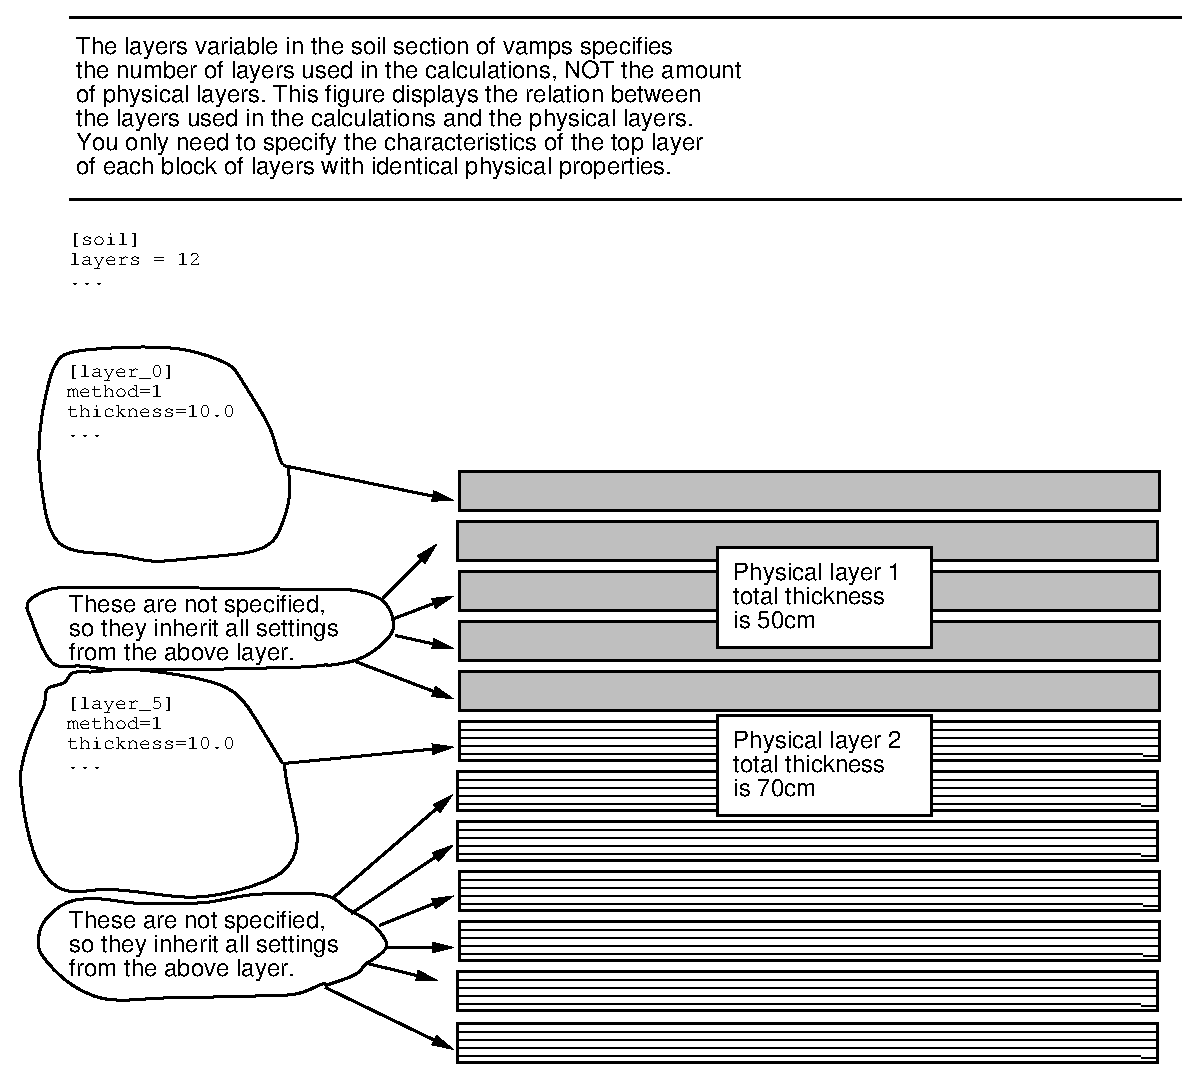
\includegraphics{psfig/layers.eps}}
\caption{Relation between the layers variable in the soil section and
the amount of physical layers.}
\label{fig:layers}
\end{figure}


\chapter{The input file}

\section{introduction}

\vamps\ reads it's options and  most of the  data needed for  modelling
from the input file. This file is in plain ascii format and is divided in
several sections. The exact format of this file is described in
section~\ref{sec:inputfileformat}.  An input file must be created before
running \vamps.  There are two way of creating an input file for \vamps.
{\em (1)} Use the (not finished) \vamps\ preprocessor. This
preprocessor\footnote{The use of this preprocessor is described in a
seperate manual} will let you choose from menu items to select all the
options that are set in the input file and generate an input file for you
once you are finished. Or you can {\em (2)} use an ascii editor or a
word-processing package to create this file.



\section{Input file format}\label{sec:inputfileformat}
The input file format for \vamps\ is much like Microsoft Windows {\tt .ini}
files.  All names and sections are case insensitive.  The case of string
variables is unaltered so filenames are case-sensitive if the operating
system is. The file is divided into sections which each contain variables
that have some connection with each other.  Each variable name is followed
by an equal sign ({\tt =}), after which the value of the variable is placed.
Example:

\begin{verbatim}
[vamps] 
verbose = TRUE 
# This is a comment

[environment]
caseid = Interception test file. Bisley catchment.\
Summer of 1995
\end{verbatim}

The \verb \ character may be use to break up long strings over more
than one line\footnote{The character itself is converted to a
space}. The \verb # sign at the start of a line is used to denote a comment
Only the first '=' sign is significant. Spaces within the names are
copied verbatim, and thus become part of the name. This makes the
following construction legal:
\begin{verbatim}
[vamps]
output mode = This is ('=') a nonsense\
example.
\end{verbatim}

In this case the variable 'name' in section 'vamps' is 'output mode'
and it's value is 'This is ('=') a nonsense example'.

\footnote{If you want you can change this character using the 
\inivar{commentchar} variable in the \inisec{vamps} section or the -C
command-line option.  Usually there should be no reason to do so}.

\vamps\ uses six types of variables: {\em (1)} \Index{floats} (floating point
numbers), {\em (2)} \Index{arrays} (a row of floating point numbers
separated by whitespace), {\em (3)} \Index{strings} (a series of
characters), {\em (4)} \Index{integers} (whole signed numbers), {\em
(5)} \Index{characters} (a single printable character) and {\em (6)}
\Index{boolean} (special kind of integer, either 0 or 1 -- FALSE of TRUE, NO or YES).


\section{Available sections and variables}\label{sec:sections}
All sections with available variables and their defaults values as
well as the type of the variable are listed below.  The most up to
date list is presently found in the {\bf vamps(5)} manual page.  You
will need this list badly when you construct an input file for
\vamps\. Once the graphical preprocessor is finished things will
become a little easier.

\vamps\ has been developed using the {\bf swap94} {\sc Fortran} code as a 
starting point.  Most names of variables have been changed (sorry) but
some of the variable names as well  as their physical meaning have not
been altered.


\subsection{[vamps]}\label{section:defaults}
\begin{description}
\item[verbose] If set to FALSE \vamps\ will be  silent, if set to
TRUE \vamps\ will display progress information

\item[header]\footnote{See also the -\,-Header option in \vamps\ (1)}
Is set to FALSE  no header in will be added to the output, if
set to TRUE an  header will be added to the output. Defaults is FALSE

\item[logging] FALSE = no logging is done, TRUE = logging is on

\item[logfilename] name of the file to which logging is performed

\item[iniinmem]
TRUE = the input file is read into memory (some speedup), FALSE = the
input file is not read into memory

\item[progstr]
String which is used to display progress information (use 0, 1 or 2
for build in strings).  0 will show calculation time and estimated
time to go. 1 will show a percentage finished bar and 2 will show
'calculating'.

You can define your own such as:
\begin{quote}
{\tt Vamps is running, please wait......................}
\end{quote}

%\item[showgraph] TRUE = if you are running UNIX and X11 or OS/2 and 
%{\tt gnuplot} is installed program progress is displayed graphically.
%FALSE = no graphical progress information.

\item[graphcommand] full path to {\tt gnuplot}
with optional command line options. In OS/2 only gnuplot.exe should be
specified here. This seems to be a 'bug' in the emx library which I used
to make the binaries.

\item[commentchars]
Character(s) that denotes the start of a comment. This defaults to \#\%
and the first character should {\em not} be changed unless you have a
very good reason to do so.

\item[xtrasl]
comma seperated  list of \slang\ files to be loaded a startup
\end{description}

\subsection{[time]}\label{section:time}

\vamps\ will not run without a time section in the input file with at
least the \inivar{steps} variable set\footnote{This will change in the beta
version in which time-steps will be determined by the time column in the
input file}.  

\begin{description}
\item[steps] Integer value specifying the number of steps in the 
current simulation.  This value should be smaller or equal to the
number of entries in the precipitation file.

\item[startpos] Position (line) in the precipitation input file used as
start. Counting starts at zero.

\item[starttime] 
day at which the simulation should start If this value is not
specified simulation starts at the first step in the precipitation
input file.  If both starttime and startpos are specified starttime
will be used.
\end{description}

\subsection{[run]}
\begin{description}
\item[outputfile]
Filename to save output to. You can override this with the \-o command
line option.

\item[runid]
No used at moment
\end{description}

\subsection{[xout]}\label{section:xout}
\begin{description}
\item[filename]
Filename for extra output in column type format. No extra output is generated if
this variable is not present.
\end{description}


\subsection{[determine]}\label{section:determine}

\begin{description}
\item[canopy]
determine canopy (see section canopy)

\item[evaporation]
determine actual evaporation (see section evaporation)

\item[pevaporation]
determine potential evaporation (see section pevaporation)

%\item[interception]
%determine interception (see section interception)

\item[soilmoisture]
determine soilmoisture profile (see section soil)

\item[fit]
Use non-linear regression to try and fit to measured data (see fit section)
\end{description}

\subsection{[pevaporation]}\label{section:pevaporation}
\begin{description}
\item[method]
0 = potential evaporation via Penman E0 (Need: refrad, netrad, rhumid,
windspeed, temp, inrad),
1 =  potential evaporation   via  Penman E0 (using   sunratio)  (Need:
sunratio, rhumid, windspeed, temp, inrad),
2 and 3 = not yet done,
4 =  potential evaporation using    Makkink (Need: rhumid,  windspeed,
temp, inrad)
\end{description}

\subsection{[evaporation]}\label{section:evaporation}
\begin{description}
\item[method]
0 = evaporation equal to potential evaporation,
1 = multiply potential evaporation by a crop factor (need cropfac),
2 = calculate actual evaporation using the Penman-Montheith formula

\item[cropfac]
A  floating point number  representing the crop  factor with which the
potential evaporation is to be multiplied to yield actual evaporation.
\end{description}

\subsection{[interception]}\label{section:interception}
\begin{description}
\item[method]
0, 1 , 2, 3.
gash, rutter laifrac or calder

\item[gamma]
gamma in calder equation

\item[delta]
delta in calder equation

\item[E\_avg/R]
Evaporation/Average Rainfall during a storm   in gash. If this is  not
set penman/Montheith will be used with $R_a$ set to zero.

\item[p\_tr]
Fraction of water diverted to the trunk (gash, rutter)

\item[p\_f]
Free throughfall coefficient (gash, rutter)

\item[S]
Canopy storage in cm (gash, rutter)

\item[gashm]
Either 1 or 0. If set to 1 an adapted version of gash is used. This
version should work for time-steps smaller then 1 day. Default = 0

\item[laifrac]
the canopy interception coefficient

\item[lai]
The canopy leaf area index. This is needed for the laifrac method. If
it is not present it is searched in the canopy section.
\end{description}


\subsection{[canopy]}\label{section:canopy}

Although you don't have to use the canopy module it is recommend that
you do so if possible. The other methods of determining transpiration,
interception etc. don't have a close interaction with the soil modules
and usually provide poorer results.


\begin{description}
\item[layers]
Number of canopy layers (this is largely determined by the accuracy of your
LAI profile). At the moment only one layer is allowed.

\item[Rnet\_absorb]
The fraction of the total radiation absorbed by the canopy ($0\le
Rnet\_absorb \le 1$). The remaining amount will be used for soil
evaporation.

\item[transpiration]
Which transpiration equation should be used.
\\
2 = penman Montheith
\item[z]
Height of the canopy (m)

\item[z\_0]
Aerodynamic roughness length (m)

\item[d]
Zero plane displacement length (m)

\item[rs]
Canopy resistance (s/m). If this is not specified the user defined regression 
equation {\bf estrs()} will be used.

\item[drytime]
If this variable is set this value (in days) will be used to determine
how long it takes for the canopy to dry. 

\item[wetevap]
If this variable is set this value (in cm/day) will be used to determine
the canopy wat evaporation rate in stead of Penman-Montheith with
Rs set to zero.
\end{description}

\subsection{[roots]}\label{section:roots}
\begin{description}
\item[depth]
depth of the root zone in cm. If you want rooting depth to change in
time you should use the \inivar{drootz} variable in the \inisec{ts}
section.

\item[swsink]
0 = sink term according to Feddes. (Need: hlim1 hlim2u hlim2l hlim3h
hlim3l hlim4)\\ 
1 = sink term according to Hoogland. (Need: hlim1
hlim2u hlim2l hlim3 hlim4) 

\item[swhypr] 0 = linear relation between
the points hlim3 and hlim4 of the sink term.\\
1 = hyperbolic
relation between the points hlim3 and hlim4 of the sink term.

\item[swupfu]
0 = water uptake function according to Feddes.\\
1 = water uptake function according to Hoogland.\\
2 = water uptake function according to Prasad (1988).

\item[cofsza] Intercept a in Feddes et. al 1988 (only needed if swupfu =1).

\item[cofszb] Slope b in Feddes et. al. 1988. (only needed if .B swupfu =1).

\item[hlim1] 
Pressure head value (cm) below which roots start to extract water from
the upper soil layer (starting point).

\item[hlim2u]
Pressure head
value (cm) below which roots start to extract water optimally from the
upper soil layer.

\item[hlim2l] 
As above, but for all lower soil layers.

\item[hlim3h]
Pressure head value (cm) below which roots cannot extract water
optimally any more, for a High pot. transpiration rate equal to 0.5
cm/d (limiting point).

\item[hlim3l] 
As above, but for low pot. transpiration rate equal to 0.1 cm/d.

\item[hlim3]
Pressure head value (cm) below which roots cannot extract water any
more (limiting point).

\item[hlim4]
Pressure head value (cm) below which no water uptake by roots is
possible (wilting point).
\end{description}

\subsection{[ts]}\label{section:ts}
The ts section has one entry that {\em must} be present:
precipitation.  The precipitation file is important because it also
determines the time-steps at which output is calculated. More
information about time-steps can be found in
section~\ref{sec:tstep}. 
\begin{figure}
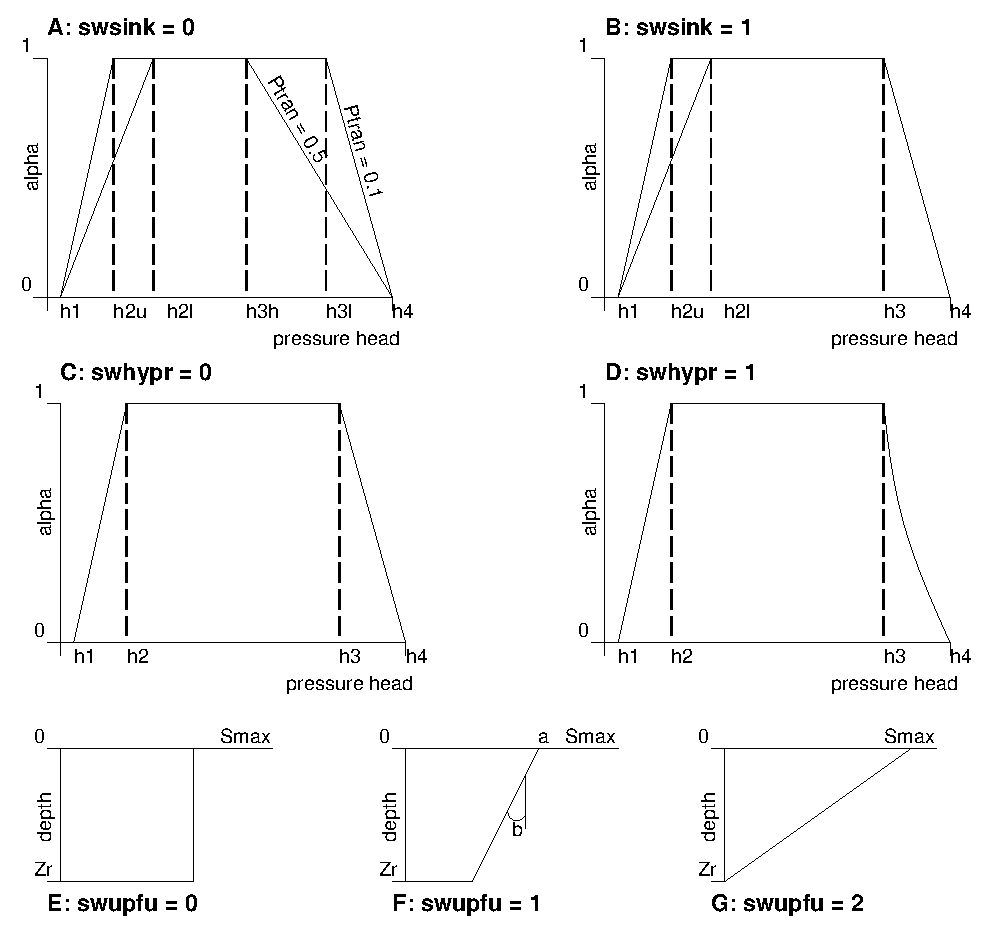
\includegraphics{psfig/soilr.eps}
\end{figure}

The file format consists of colums separeted by whitespace (space
or tabs).  \vamps\ assumes the first column to hold the time and the
second column to hold the value. You can override these assumptions by
appending {\tt ,xcol,ycol} to the filename\footnote{This implies that a comma
is {\em not} allowed in a filename}. Counting begins at zero.

The ts section can be handy if you don't like the method(s) which
\vamps\ can use for determining things like potential evaporation.
Simply put them in here and \vamps\ will use the values you supplied
instead.

\begin{description}
\item[pevaporation]
Name of file with potential evaporation data (if not calculated)

\item[ptranspiration]
Name of file with potential transpiration data (if not calculated)

\item[interception]
Name of the file with interception data (if not calculated)

\item[precipitation]
Name of file with precipitation data. This file file also determines
the time-steps at which output is calculated. See section~\ref{sec:tstep}
for more information.

\item[drootz]
Name of file with rooting depth (cm) in time. You need to specify at
least three points. Other points will be interpolated using a spline
if they don't exist. See the file {\tt src/tc/ts\_spl.c} for the
interpolation routine.
\end{description}

\subsection{[soil]}\label{section:soil}
\begin{description}
\item[outskip]
Skip outskip timesteps in soil output. Used to reduce
outputfile size.

\item[initprof]
0 = water content profile (need theta\_initial array),
1 = pressure head profile (need h\_initial array) and
2 = Calculate pressure head profile (need gw\_initial in soil section).

\item[gw\_initial]
initial ground-water level in cm below field-level (needed if 
initprof = 2)

\item[swredu]
Reduction of soil evaporation \\
0 = no reduction, 1 = the Black (1969) model is used,
2 = the Boesten (1986) model is used and
3 = an adapted version of the Boesten (1986) model is used. 
This version takes into
account the actual moisture condition of the soil surface.

\item[cofred]
The factor alfa in Black or Beta in Boesten. This is not needed for
swredu = 0.  
\item[bottom]
Bottom boundary condition:
0 = daily ground-water table depth (cm) is input,
1 = Given flux,
2 = seepage or infiltration from/to deep ground-water,
3 = Flux calculated as a function of h,
4 = interpolation between daily values of given pressure head,
5 = Zero flux at bottom,
6 = Free drainage.

\item[smooth]
Integer value giving the size of the running average used for smoothing 
the ksat, theta\_saturation and residual\_water profile. 
Set to zero for no smoothing (default).

\item[layers]]
Number of soil layers in calculation (how many real (physical) layers
exist is specified by the amount of layers\_{\em n} sections\footnote{
see also section~\ref{sec:physlay} on page~\pageref{sec:physlay}})

\item[pondmx]
Maximum amount of ponding (in cm) allowed at the top of the profile,
defaults to 0.0.

\item[gwlevel]
Water level at bottom of profile, needed
if bottom = 4 

\item[dtmax]
Maximum time-step (in days) in soil module

\item[dtmin]
Minimum time-step (in days) in soil module. Both dtmax and dtmin
should probably be left alone. By setting dtmin and dtmax to the 
same value \vamps\ can be forced to use a fixed time-step.


\item[speed]
Integer value ranging from 1 (slow) to 6 (fastest) determining
the tradeoff between calculation accuracy and speed. This options
combines the settings in dtmin, thetol, solvemet, mktable,
maxitr and swnums.

If you also specify one of these variables seperately the settings
from speed are overridden. Default  for speed is 3.

\item[maxitr]
Maximum number of iterations in the soil module. Iterations
are only performed if swnums == 1.

\item[thetol]
Theta tolerance. If swnums != 1 (by default) 
\vamps\
will use this value to check if the solution is good enough and
perform iterations if needed. Setting this value to high or low
gives poor results. The default value usually works fine. If
you have no problems you better leave this one alone. Usually
this variable should be between 1.0E-2 and 1.0E-5.

\item[solvemet]
Determines how vamps solves the equation matrix.
If set to 0 the default (tridiagonal) solution is used.
If set to 1 the soil module will always treat the solution as a band-diagonal
matrix. If set to 2 a very general solution is used. This solution
includes a step to regain full machine precision but is rather slow.

\item[swnums]
If set to 1 the soil module won't check for convergence of solution.
It assumes that the initial maximum dt is a good guess. Things can be
quit a lot faster in all cases but can give poor results in most cases
as well.

\item[mktable]
if set to true 
\vamps\
will create look up tables for the theta vs K relation, and use those
in stead of the function during iteration.  By default this option is
set to false. Set to true to speed up calculation. The solution can
become instable at high suction heads. In stead of letting 
\vamps\
generate the look-up tables you can also read pre-made tables
using the method option in the layer\_n section.


Depending on the problem, the amount of memory you have installed, the
floating-point performance of you CPU and the optimizations your
compiler can make, this can speed up calculations by 50\%. You will
lose some precision in the process. By default the program uses 300
points long look-up tables. Use the \inivar{tablesize} variable in the
\inisec{soil} section to change this value.

There is no exact way to determine the speed increase you will
get. For example, on a 66MHz 486DX2 running Linux, a 25\% speed
increase was established without compiler optimization (gcc) while a
50\% speed increase was measured when de program was compiled with
optimization. It seems that gcc does a better job optimizing the look
up procedure than the intensive floating point calculations in the van
Genuchten equation\footnote{actually the all important thing here is
how fast your compiler/CPU combo can execute the pow() function
as this usually account for 90\% of the CPU time!}. 
On a RISC processor with better floating point
performance this balance may be different, and you probably won't get
speed increases of 50\%. On a rs6000 365 running AIX 3.2 the mktables
option resulted in a 23\% speed increase.

\item[estdmc]
if set to true and the \inivar{mktable} variable is also true the dmc
table will be made using ts\_slopes and the Pf curve in stead of the
\slfunc{h2dmc} function. If you use \slang\ soil functions and you define
\inivar{estdmc} to be true you don't need the \slfunc{h2dmc} function.


\item[tablesize]
Sets the size of the look-up tables. Defaults to 300. Increase this
for better accuracy at a penalty of using more memory and some
performance loss. Provided the program fits in physical memory table
sizes up to 1200 (very large) points still give some speed
improvements compared to not using the look-up tables.  Sometimes
decreasing this to 80 or so can be done without much loss of accuracy
or stability.

\item[dumptables]
If set to true the look up tables will be dumped to the initial
section of the output-file; x and y in separate array type  variables for each
layer. This can be handy for plotting pF curves for example.

\item[verbose]
Verbose level in soil module (0 = silent). I recommend a setting
of 1 (default) which will show you how long \vamps\ will run.

\item[smddepth]
If this variable is set the SMD (soil moisture deficit) will
be calculated until this depth. Otherwise the rooting depth
will be taken.
\item[fieldcap]
Head in cm at which the soil is at field capacity. Needed for
determination of soil moisture deficit. Default = -100.0

\end{description}

\subsection{[drainage]}\label{section:drainage}
This is presently in a very experimental stage. One day when \vamps\
will be two-dimensional this will become more important.

\begin{description}
\item[method]
Variable which controls the type of lateral drainage.\\
\centerline{
\begin{tabular}{ll}
Value & Description \\ \hline
0 & No lateral drainage (default) \\
1 & TOPOG type drainage (only at saturation) and \\
2 & Allow also unsaturated lateral flow \\
\end{tabular}}
If the \inivar{drainage} variable is larger than zero the
\inivar{slope} variable must be set also.

\item[slope]
Slope used in the calculation of lateral drainage (floating point value).
 
\item[exclude]
Array with layers in which lateral drainage is not allowed. 
0 <= value < layers  
example:
\begin{verbatim}
exclude = 12 1 23 45
\end{verbatim}
You can use a construction like this and a no-flow bottom boundary
to simulate a lysimeter.

\end{description}

\subsection{[{\em soilsectionname}]}\label{section:soilsectionname}
This section can have {\em any} name and contains the soil specific
info.  The \inivar{soilsection} variable in the \inisec{layer\_n}
section refers to the name of this section.

\begin{description}
\item[method]

Method for k vs theta relation:\\
\centerline{
\begin{tabular}{ll}
Value & Description \\ \hline
0 & clapp/hornberger\\
1 & van Genuchten\\
2 & not yet implemented\\
3 & van Genuchten parameters are determined from theta vs pf
pairs\\
4 & read TOPOG \_soil soil tables\\
5 & user defined S-Lang functions\\
\end{tabular} 
}

\begin{description}
\item[ad 3)] Given values of alpha and n are used as initial
guesses. Required variables: \inivar{theta} (array of values) and
\inivar{pf} (array of values). Optional: \inivar{alpha} and \inivar{n}.  
The exponent l is set to 0.5,

\item[ad 4)] \vamps\ has the ability to read
and use soil tables generated by the TOPOG \_soil program. It will
then use these look-up tables in stead of using direct
calculations. In future \vamps\ will be distributed with it's own
version of the \_soil program

\item[ad 5)]
In this case the user must define the following S-Lang functions:

\vspace{0.5cm}
\centerline{
\begin{tabular}{ll}\hline\hline
  Function & Description \\ \hline
  {\tt Void getspar(char *section, Int nr)} & \parbox[t]{4.5cm}{called to get additional parameters from the input file} \\
  {\tt Float h2dmc(Int nr, Float head)} &  \parbox[t]{4.5cm}{calculates suction head to differential moisture capacity} \\
  {\tt Float t2k(Int nr, Float theta)} & \parbox[t]{4.5cm}{calculates $k_{unsat}$ from moisture content (theta)} \\
\parbox[t]{6.5cm}{\tt Float t2h(Int nr, Float theta, Float depth)} & \parbox[t]{4.5cm}{calculates suction head from  moisture content (theta)} \\
  {\tt Float h2t(Int nr, Float head)} & \parbox[t]{4.5cm}{calculates moisture content from suction head} \\ \hline
\end{tabular}
}\vspace{0.5cm}

If you use this option you should either have a {\em very} fast computer or
use the \inivar{mktable} option in the \inisec{soil} section. The following
tables list some example excecution time when using the some method coded
in C and \slang{}.

\vspace{0.5cm}
\centerline{
\begin{tabular}{ll}\hline \hline
Method & time [sec] \\ \hline
C -- no tables & 25.37 \\
C -- tables & 18.52 \\
SL -- no tables & 393.90 \\
SL -- tables & 19.49 \\ \hline
\end{tabular}
}\vspace{0.5cm}

An example can be found in the file func.sl in the vampslib directory.
\end{description}

\item[description]
An optional description of the soil layer.

\item[ksat]
Saturated hydraulic conductivity of the layer.

\item[kh/kv]
Ratio of $K_{sat}$ horizontal divided by $K_{sat}$ vertical. This
is only used if you use lateral drainage (see drainage section).
By default this is set to one.

\item[thetas]
Theta at saturation (porosity).

\item[psisat]
Head at saturation (air entry value) needed for Clapp/Hornberger

\item[b]
Factor b in Clapp/Hornberger

\item[theta\_residual]
Residual amount of soil moisture.

\item[alpha]
Alpha in van Genuchten.

\item[l]
l in van Genuchten (use 0.5 if not determined). Normally (unless you
have determined a theta vs $K_{unsat}$ relation) you don't
have this information.

\item[n]
n in van Genuchten.


\item[tablefile]
File from which the soil table should be read. Use this if method = 4.

\item[tablefiletype]
Type of the table-file. All filetypes can have comment-lines starting with \#.
\\
\centerline{
\begin{tabular}{ll}
Value & Description \\ \hline
1 & TOPOG-type \vamps\ only uses columns 1, 3 4 and 5\\
2 & White space separated columns (psi theta k)\\
3 & White space separated columns (psi theta k diff\_moist) \\
\end{tabular}
}
ad 2) In this case the differential
moisture capacity (d\_theta/d\_phi) is estimated.

Note that all tables should be made with {\em descending}
theta values.
\end{description}

\subsection{[layer\_{\em n}]}\label{section:layers}
Only the \inisec{layer\_0} section is a must. The rest is only needed if you
have more than one physical soil layer.

\begin{description}

\item[thickness]
Thickness of the layer (in cm).

\item[soilsection]
Name of the section that contains the soiltype info for this layer (node).

\end{description}

\subsection{[fit]}\label{section:fit}
\begin{description}
\item[fit]
Data-set used in fitting

\item[fitto]
Name of a time serie (must be specified in the ts section) with
actual measurements

\item[n]
(n = 0 ... n= MAXPAR)
Add a new parameter to the fitting list.
At present the following
parameters are available:
\\
1 (n)
\\
2 (alpha)
\\
3 (ksat)
\\
4 (b)
\\
5 (psisat)
\\
6 (l)
\\
7 (residual\_water)
\\
8 (thetas)

\item[layer]
Physical layer to use in fitting.
\end{description}



\subsection{Valid datasets}
\vamps\ recognizes the following datasets:\footnote{Used in the ts section
and the -\,-Output option.}
\begin{itemize}
\item[pre] precipitation [cm]
\item[rlh] relative humidity [%]
\item[hea] head at bottom [cm] 
\item[rdp] rooting depth [cm] 
\item[tem] dry bulb temp [oC] 
\item[gwt] ground-water table [cm] 
\item[inr] interception [cm] 
\item[trf] troughfall   [cm] 
\item[stf] stemflow     [cm] 
\item[pev] potential evaporation [cm] 
\item[spe] potential soil evaporation [cm] 
\item[ptr] potential transpiration [cm] 
\item[qbo] flow through bottom of profile [cm] 
\item[vol] actual water content [cm] 
\item[avt] average theta in profile 
\item[lai] leaf area index 
\item[sca] canopy storage [cm???] 
\item[ira] incoming radiation [W/m2] 
\item[nra] net radiation [W/m2] 
\item[ref] reflected radiation [W/m2] 
\item[win] windspeed [m/s] 
\item[sur] sunratio [n/N] 
\end{itemize}

\section{Interception}
\vamps\ can determine interception loss via several methods. The
Calder method \cite{calder1986171}, the Gash analytical method (see
paragraph~\ref{par:gash}) and Rutter's
\cite{rutter1971174} numerical method. For the Rutter method you will need
precipitation data with hourly or shorter intervals.  All parameters
needed for interception calculation are set in the interception section
of the input file. Each method has it's own set of required and optional
arguments. In addition you also need at least one time-series
(precipitation). Figure~\ref{fig:ex:gash} and Figure~\ref{fig:ex:calder}
show a part of a input file which calculates interception using the Gash
and the Calder method respectively. A description of all allowed variables
in the interception section is given in section~\ref{sec:sections} on
page~\pageref{section:interception}.

%-----------------------------------------------------------------------
\chapter{Running \vamps}
Although you don't have to use the canopy module it is recommend that
you do so if possible. The other methods of determining transpiration,
interception etc. don't have a close interaction with the soil modules
and usually provide poorer results.


\section{Command line options}
Options may be given as either standard one-letter options, or GNU style
long options. Long options start with two dashes '\-\-' and may be truncated
to any unambiguous abbreviation.

\begin{description}
\item[-\,-Header]
Omit the headers in output.

\item[-\,-copyright]
Show copyright information and exit

\item[-\,-license]
Print license information and exit.

\item[-\,-help]
Print help text and exit.

\item[-\,-verbose]
Enter verbose mode, program progress is displayed on stderr.
Default is silent.

\item[-\,-noinputdump]
By default the contents of the inputfile is also included in the 
output. Use this option to alter this behaviour.

\item[-\,-Output  {\em setname}]
Dump the specified 
{\em setname}
to a seperate file in
{\bf ts}(5)
format. See
{\bf vamps}(5)
for a list of allowed setnames.

\item[-\,-Determine {\em variable}]
Determine variable (can be a single variable or a time series).
See {\bf vamps}(5)
for a list of allowed variables.

\item[-\,-Logfile {\em filename}]
Log this session to the file {\em filename}.

\item[-\,-Setvar {\em section name value}]
Set the value of variable {\em name}
in section {\em section} to value {\em value}.
This overrides the setting in the input file.

\item[-\,-Comment {\em commentchar}]
Set the commentchar to char {\em commentchar}.

\item[-\,-showdef]
Send program defaults to stdout. This can be used to create a
default file from scratch.


\item[-\,-output {\em filename}]
Send output to {\em filename}
in stead of stdout.

\item[filename]
Read input from {\em filename}
\end{description}

\section{Manipulation of time series}
Links to the ts*(1) stuff

\section{graphically displaying \vamps\ results}
Links to the graph(1) stuff


\section{Troubles..}\label{sec:troubles}
OK, you have problems running \vamps. You are not alone!
I will describe some problems that you can encounter
using \vamps. Some have an easy solution, others not.

\subsection{Variable missing}
If \vamps\ issues a message like:

\begin{verbatim}
deffile.c: Fatal:	could not find	->steps<-
	in section		->time<-
	in file			->example1.inp<-
deffile.c:	error message:
	from: $Id: deffile.c,v 1.23 1996/03/18 09:24:50 schj Exp $
	description: Var not found or invalid, see above.
\end{verbatim}

you have not specified a variable in the input file which \vamps\ {\em
needs} to run properly. This can be a variable which is needed always
or one that is needed is you have specified so in an other variable.
For example, if you specify the Gash method for determining interception
you {\em must} also specify the variable \inivar{S} in the \inisec{interception}
section.


\subsection{Mass-balance error warning}

\vamps\ issues a warning when large jumps in the mass-balance error
are encountered. You can ignore them providing you keep in mind that
the solution is not very optimal. At present the mass-balance is {\em
not} calculated properly is you use lateral drainage, beware! In most
circumstances decreasing the \inivar{dtmax} variable helps, it 
prevents \vamps\ from making mistakes in estimating the max timestep.
Descreasing the \inivar{dtmin} and/or the \inivar{thetol} variable should
be next on your list followed by increasing the \inivar{maxitr} variable.



%--------------------------------------------------------------------------
\chapter{Using \slang{} with \vamps{}}

\section{Introduction}
To allow users to change functions that \vamps\ uses to determine
like converting incoming radiation to net radiation as well as other
emperical equations, \vamps{} includes the \slang{} stack based
interpreter. \citeasnoun{davis1995282} describes \slang{} as:
\begin{quote}
\slang{} (pronounced ``sssslang'') is a powerful stack based interpreter
   that supports a C-like syntax.  It has been designed from the beginning
   to be easily embedded into a program to make it extensible. \slang{} also
   provides a way to quickly develop and debug the application embedding it
   in a safe and efficient manner.  Since \slang{} resembles C, it is easy to
   recode \slang{} procedures in C if the need arises.
\end{quote}
The actual syntax of \slang{} is not described here -- see
\cite{davis1995282,davis1995283} for that -- but the way \vamps{} uses
\slang{} for it's extensions. Also \vamps{} specific \slang{} functions
and variables are described here.


\section{How \vamps{} interfaces with \slang{}}

For speed reasons \vamps\ only uses the \slang{} interpreter at
specific locations in the program:

\begin{enumerate}
\item at startup \vamps\ loads a file (usually {\tt vamps.sl}) with
the function definitions of functions that \vamps\ uses.
\item at the start of the program -- after the input file is read -- \vamps\
executes the {\tt at\_start} function
\item after each timestep the {\tt each\_step} is executed
\item after all calculations are done -- but before data is flushed
from memory -- the {\tt at\_end} function is executed
\item a series of regression equations and relations between variables
can be programmed in \slang{}. \vamps\ checks is a certain \slang{} function
exits and executes that in stead of the build in function. at present the
following functions can be programmed in \slang{}:
\begin{itemize}
\item {\tt lai\_to\_s (lai)} -- returns s (canopy storage) for a given lai (leaf area
index)
\item ......
\end{itemize}
\end{enumerate}



\chapter{\vamps\ specific functions and variables}
\section{Intrinsic functions (programmed in C)}
% Generated by sldoc.slx (1.14, (C) 1996, 1997) Tue Dec 16 10:54:34 1997


\paragraph{\index{\#}\#}
\begin{verbatim}
# [plotcommand]
\end{verbatim}
Operator to send a single command to the plotting system (gnuplot) when
followed by an argument or to enter plotting mode if no argument is given.
In plotting mode all commands should be gnuplot commands. To switch back to
normal mode give a single '\#'. The {\tt :} and \verb1\1@ operators also work within
plotting mode.


Some special characters can be used to addres S-Lang variables from within
plotting mode. Words withing \$'s are replaced by a string representation of
the S-Lang variable with that name. Example
\begin{verbatim}
variable h = "sin(x)";
# plot $h$
\end{verbatim}
To plot S-Lang matrix variables the \verb1\1@ char must be used. Example
\begin{verbatim}
variable m = mread("mydata.file",-1);
# plot @m@ using 1:2
\end{verbatim}
Although S-Lang matrix variables are zero based gnuplot starts counting at
1.


Variables from vamps output files can also be plotted. In this case both
the name of the of the variable and the output filename are needed.
They should be seperated by a colon and enclosed in \verb1\1@ characters:
\begin{verbatim}
# plot @precipitation:example1.out@ using boxes
\end{verbatim}
See also {\tt plt}.


from: {\tt ..$/$src$/$main$/$init\_s.c}

from file: {\tt intrin.doc}


\paragraph{\index{:}:}
\begin{verbatim}
: command [options ...]
\end{verbatim}
Execute a system {\tt command} in a subshell. Note that the
syntax does not use S-Lang conventions; everything after
the `{\tt :}' is passed to the shell. Returns nothing, a message
is printed on standard error if {\tt command} returned a non-zero
exit status.


from: {\tt ..$/$src$/$main$/$intrins.c}

from file: {\tt intrin.doc}


\paragraph{\index{?}?}
\begin{verbatim}
? [name ...]
\end{verbatim}
Invoke the {\tt vamps} online help system. This command can
only be used when running interactive.


If a single `{\tt ?}' is entered at the prompt, a list of
{\tt names}, typically {\tt vamps} command or variable names, for
which online documentation is present will be printed on
the screen.


If one or more {\tt name}(s) are given after the `{\tt ?}', the
available documentation text for those {\tt name}(s) is printed
on the screen.


If there is more than one screenfull of text, the {\tt cursor}
and {\tt PgDn$/$PgUp} keys will cause the text to scroll; pressing
`{\tt q}' will stop text display and go back to the command
prompt.


from: {\tt ..$/$src$/$main$/$intrins.c}

from file: {\tt intrin.doc}


\paragraph{\index{@}@}
\begin{verbatim}
@scriptname
\end{verbatim}
This operator passes it's argument to {\tt evalfile}. It
can only be used when running interactively. It
can be used to run scripts in stead of an expression
like:
\begin{verbatim}
() = evalfile("scriptname");
\end{verbatim}
Note the lack of a space between the operator and it's
argument!


from: {\tt ..$/$src$/$main$/$init\_s.c}

from file: {\tt intrin.doc}


\paragraph{\index{SLang\_init\_tty}SLang\_init\_tty}
\begin{verbatim}
Int SLang_init_tty()
\end{verbatim}
Initialize the S-Lang tty. 


from: {\tt ..$/$src$/$main$/$init\_s.c}

from file: {\tt intrin.doc}


\paragraph{\index{SLang\_reset\_tty}SLang\_reset\_tty}
\begin{verbatim}
Int SLang_reset_tty()
\end{verbatim}
Resets the S-Lang tty. Needed is you want to use stdin and
stdout from interactive mode.  


from: {\tt ..$/$src$/$main$/$init\_s.c}

from file: {\tt intrin.doc}


\paragraph{\index{Slai\_to\_s}Slai\_to\_s}
\begin{verbatim}
Float Slai_to_s(Float lai)
\end{verbatim}
Function called in the canopy module to convert lai to
canopy storage. If this S-Lang function is not defined the
lai value from the {\tt canopy} section in the input file is used.


from: {\tt ..$/$src$/$main$/$init\_s.c}

from file: {\tt intrin.doc}


\paragraph{\index{\_sets\_}\_sets\_}
\begin{verbatim}
Int _sets_
\end{verbatim}
Number of data sets in memory 


from: {\tt ..$/$src$/$main$/$init\_s.c}

from file: {\tt intrin.doc}


\paragraph{\index{\_version\_}\_version\_}
\begin{verbatim}
Int _version_
\end{verbatim}
Devide by 10 to get version number of Vamps 


from: {\tt ..$/$src$/$main$/$init\_s.c}

from file: {\tt intrin.doc}


\paragraph{\index{addset}addset}
\begin{verbatim}
Void addset(name, points)
\end{verbatim}
Adds an empty set {\tt name} with {\tt points} points
to the list


from: {\tt ..$/$src$/$main$/$init\_s.c}

from file: {\tt intrin.doc}


\paragraph{\index{addtohist}addtohist}
\begin{verbatim}
Int addtohist(string)
\end{verbatim}
Adds {\tt string} to the history list.


from: {\tt ..$/$src$/$main$/$init\_s.c}

from file: {\tt intrin.doc}


\paragraph{\index{arg0}arg0}
\begin{verbatim}
String arg0
\end{verbatim}
Readonly variable holding the name of the application
(``{\tt slash}'' if running interactive) or the name of the
current script file being processed.


from: {\tt ..$/$src$/$main$/$intrins.c}

from file: {\tt intrin.doc}


\paragraph{\index{closedef}closedef}
\begin{verbatim}
int closedef ()
\end{verbatim}
Description: closes a file previously opened with opendef
Returns: fclose's result


from: {\tt ..$/$src$/$deffile.lib$/$sl\_inter.c}

from file: {\tt intrin.doc}


\paragraph{\index{cont}cont}
\begin{verbatim}
cont()
\end{verbatim}
Continiue the current Vamps run 


from: {\tt ..$/$src$/$main$/$init\_s.c}

from file: {\tt intrin.doc}


\paragraph{\index{copyright}copyright}
\begin{verbatim}
Void disclaim
Void copyright
\end{verbatim}
Shows a short version of the GPL 


from: {\tt ..$/$src$/$main$/$init\_s.c}

from file: {\tt intrin.doc}


\paragraph{\index{cpu}cpu}
\begin{verbatim}
Float cpu()
\end{verbatim}
Return the number of CPU seconds used since the start of
the program. On msdos systems this will be equal to the
total run-time. On multitasking systems the actually used cpu time
will be returned.


from: {\tt ..$/$src$/$main$/$init\_s.c}

from file: {\tt intrin.doc}


\paragraph{\index{defverb}defverb}
\begin{verbatim}
Int defverb
\end{verbatim}
The verbose level in the input file routines. 0 is quit. A higher
the number makes this part of Vamps more verbose 


from: {\tt ..$/$src$/$deffile.lib$/$sl\_inter.c}

from file: {\tt intrin.doc}


\paragraph{\index{disclaim}disclaim}
\begin{verbatim}
Void disclaim
Void copyright
\end{verbatim}
Shows a short version of the GPL 


from: {\tt ..$/$src$/$main$/$init\_s.c}

from file: {\tt intrin.doc}


\paragraph{\index{error}error}
\begin{verbatim}
Void error(String str)
\end{verbatim}
Prints the text held in {\tt str} followed by a newline on standard
error output and raises internal error status.


from: {\tt ..$/$src$/$main$/$intrins.c}

from file: {\tt intrin.doc}


\paragraph{\index{exit}exit}
\begin{verbatim}
exit()
quit()
\end{verbatim}
Quits the S-Lang interpreter and returns to the
operating system 


from: {\tt ..$/$src$/$main$/$init\_s.c}

from file: {\tt intrin.doc}


\paragraph{\index{exit}exit}
\begin{verbatim}
exit()
quit()
\end{verbatim}
Quits the S-Lang interpreter and returns to the
operating system 


from: {\tt ..$/$src$/$main$/$init\_s.c}

from file: {\tt intrin.doc}


\paragraph{\index{format}format}
\begin{verbatim}
Void format(String fmt)
\end{verbatim}
Sets the floating point output format to {\tt fmt}. If given
as the nullstring (""), the default format is restored.
The default can be set by calling {\tt format} from {\tt .vampssl},
else it is set to ``{\tt \%6g}''. (Using the S-Lang intrinsic
{\tt set\_float\_format} is deprecated.)


from: {\tt ..$/$src$/$main$/$intrins.c}

from file: {\tt intrin.doc}


\paragraph{\index{fscanf}fscanf}
\begin{verbatim}
..., Integer scanf(String *fmt)
..., Integer fscanf(Integer fid, String *fmt)
..., integer sscanf(String *str, String *fmt)
\end{verbatim}
Formatted variable assignment like their C counterparts
(see {\tt scanf(3)}), except that the assigned values, followed
by the number of assignments are placed on the stack. For
example:
\begin{verbatim}
    variable month, day;
    if(sscanf("December, 5\n", "%[A-Z a-z], %d\n") == 2)
    {
        (month, day) = ();
        ...
    }
\end{verbatim}
pushes a string followed by an integer on the stack.


from: {\tt ..$/$src$/$main$/$intrins.c}

from file: {\tt intrin.doc}


\paragraph{\index{getarg}getarg}
\begin{verbatim}
String getarg()
\end{verbatim}
Returns a string holding the next command line argument or
``{\tt --}'' if there are no options left. Increases the internal
index to the command line arguments each time it is called.
For example:
\begin{verbatim}
    variable arg;
    while(arg = getarg(), strcmp("--", arg))
    {
        ...
    }
\end{verbatim}
from: {\tt ..$/$src$/$main$/$intrins.c}

from file: {\tt intrin.doc}


\paragraph{\index{getdefar}getdefar}
\begin{verbatim}
String getdefstr(section, name, def, fname, exitonerror)
Int getdefint(section, name, def, fname, exitonerror)
Float getdefdoub(section, name, def, fname, exitonerror)
Int, Array getdefar(section, name, fname, exitonerror)
\end{verbatim}
A series of functions te get information from Vamps input$/$output files.


They get the value for variable {\tt name} in section {\tt section}
of the file {\tt fname}. If {\tt exitonerror} !$=$ 0 then the
program is terminated if {\tt name} is not found in {\tt section}.
If {\tt exitonerror} $=$$=$ 0 and {\tt name} is not found {\tt def} is
returned instead.
{\tt getdefar} is somewhat different. Is does not allow a {\tt def}
variable and return either one or two values. It always returns
the number of points read. If zero
points are read no array is returned.


Say we use the following file (named ex.inp):
\begin{verbatim}
[example]
examplename = nonsense
\end{verbatim}
And then call the {\tt getdefstr} function like this:
\begin{verbatim}
variable exn = getdefstr("example","examplename","Not found","ex.inp",0);
\end{verbatim}
the variable exn will now hold the string "nonsense".


from: {\tt ..$/$src$/$deffile.lib$/$sl\_inter.c}

from file: {\tt intrin.doc}


\paragraph{\index{getdefdoub}getdefdoub}
\begin{verbatim}
String getdefstr(section, name, def, fname, exitonerror)
Int getdefint(section, name, def, fname, exitonerror)
Float getdefdoub(section, name, def, fname, exitonerror)
Int, Array getdefar(section, name, fname, exitonerror)
\end{verbatim}
A series of functions te get information from Vamps input$/$output files.


They get the value for variable {\tt name} in section {\tt section}
of the file {\tt fname}. If {\tt exitonerror} !$=$ 0 then the
program is terminated if {\tt name} is not found in {\tt section}.
If {\tt exitonerror} $=$$=$ 0 and {\tt name} is not found {\tt def} is
returned instead.
{\tt getdefar} is somewhat different. Is does not allow a {\tt def}
variable and return either one or two values. It always returns
the number of points read. If zero
points are read no array is returned.


Say we use the following file (named ex.inp):
\begin{verbatim}
[example]
examplename = nonsense
\end{verbatim}
And then call the {\tt getdefstr} function like this:
\begin{verbatim}
variable exn = getdefstr("example","examplename","Not found","ex.inp",0);
\end{verbatim}
the variable exn will now hold the string "nonsense".


from: {\tt ..$/$src$/$deffile.lib$/$sl\_inter.c}

from file: {\tt intrin.doc}


\paragraph{\index{getdefint}getdefint}
\begin{verbatim}
String getdefstr(section, name, def, fname, exitonerror)
Int getdefint(section, name, def, fname, exitonerror)
Float getdefdoub(section, name, def, fname, exitonerror)
Int, Array getdefar(section, name, fname, exitonerror)
\end{verbatim}
A series of functions te get information from Vamps input$/$output files.


They get the value for variable {\tt name} in section {\tt section}
of the file {\tt fname}. If {\tt exitonerror} !$=$ 0 then the
program is terminated if {\tt name} is not found in {\tt section}.
If {\tt exitonerror} $=$$=$ 0 and {\tt name} is not found {\tt def} is
returned instead.
{\tt getdefar} is somewhat different. Is does not allow a {\tt def}
variable and return either one or two values. It always returns
the number of points read. If zero
points are read no array is returned.


Say we use the following file (named ex.inp):
\begin{verbatim}
[example]
examplename = nonsense
\end{verbatim}
And then call the {\tt getdefstr} function like this:
\begin{verbatim}
variable exn = getdefstr("example","examplename","Not found","ex.inp",0);
\end{verbatim}
the variable exn will now hold the string "nonsense".


from: {\tt ..$/$src$/$deffile.lib$/$sl\_inter.c}

from file: {\tt intrin.doc}


\paragraph{\index{getdefstr}getdefstr}
\begin{verbatim}
String getdefstr(section, name, def, fname, exitonerror)
Int getdefint(section, name, def, fname, exitonerror)
Float getdefdoub(section, name, def, fname, exitonerror)
Int, Array getdefar(section, name, fname, exitonerror)
\end{verbatim}
A series of functions te get information from Vamps input$/$output files.


They get the value for variable {\tt name} in section {\tt section}
of the file {\tt fname}. If {\tt exitonerror} !$=$ 0 then the
program is terminated if {\tt name} is not found in {\tt section}.
If {\tt exitonerror} $=$$=$ 0 and {\tt name} is not found {\tt def} is
returned instead.
{\tt getdefar} is somewhat different. Is does not allow a {\tt def}
variable and return either one or two values. It always returns
the number of points read. If zero
points are read no array is returned.


Say we use the following file (named ex.inp):
\begin{verbatim}
[example]
examplename = nonsense
\end{verbatim}
And then call the {\tt getdefstr} function like this:
\begin{verbatim}
variable exn = getdefstr("example","examplename","Not found","ex.inp",0);
\end{verbatim}
the variable exn will now hold the string "nonsense".


from: {\tt ..$/$src$/$deffile.lib$/$sl\_inter.c}

from file: {\tt intrin.doc}


\paragraph{\index{hist}hist}
\begin{verbatim}
Void hist()
\end{verbatim}
Prints the history of command entered at the interactive
prompt to the screen.


Note that the  help operator `?' is never added to the list.
The excecute operator \verb1\1{\tt  is replaced by }() $=$ evalfile("arg");@.


from: {\tt ..$/$src$/$main$/$init\_s.c}

from file: {\tt intrin.doc}


\paragraph{\index{interpreter}interpreter}
\begin{verbatim}
Void interpreter(int verb)
\end{verbatim}
Start the Vamps interactive mode. If {\tt verb} !$=$ 0
the opening banner will be shown.


from: {\tt ..$/$src$/$main$/$init\_s.c}

from file: {\tt intrin.doc}


\paragraph{\index{makeindex}makeindex}
\begin{verbatim}
Int makeindex(filename)
\end{verbatim}
Makes an index (in memory) of file {\tt filename}. It is usefull
to speed up random access to large vamps output files. Use
{\tt saveindex} to save the index to a file.


from: {\tt ..$/$src$/$deffile.lib$/$sl\_inter.c}

from file: {\tt intrin.doc}


\paragraph{\index{maqend}maqend}
\begin{verbatim}
Void maqend(int maq_m)
\end{verbatim}
Cleans up after {\tt maqinit}


from: {\tt ..$/$src$/$maq.lib$/$marquard.c}

from file: {\tt intrin.doc}


\paragraph{\index{maqhead}maqhead}
\begin{verbatim}
Void maqhead()
\end{verbatim}
prints startup options of the {\tt maqrun} procedure to
stderr


from: {\tt ..$/$src$/$maq.lib$/$marquard.c}

from file: {\tt intrin.doc}


\paragraph{\index{maqinit}maqinit}
\begin{verbatim}
Int maqinit(int m, int n)
\end{verbatim}
Initializes the fitting system. n is the number of
parameters to use, m the number of points used in the
fitting process.


Returns 0 on success, -1 on error


from: {\tt ..$/$src$/$maq.lib$/$marquard.c}

from file: {\tt intrin.doc}


\paragraph{\index{maqrun}maqrun}
\begin{verbatim}
Int maqrun()
\end{verbatim}
Runs the fitting procedure with the current settings
The S-Lang function {\tt Int fitf(Array par[], Int m, Int n)} which
sets the {\tt rv[]} array should be defined and working. It should return
0 if successfull and 1 if the function could not be resolved with
the supplied values for {\tt par[]}.


Returns 0 on success


from: {\tt ..$/$src$/$maq.lib$/$marquard.c}

from file: {\tt intrin.doc}


\paragraph{\index{maqtail}maqtail}
\begin{verbatim}
Void maqtail()
\end{verbatim}
prints exit info of the {\tt maqrun} procedure to
stderr


from: {\tt ..$/$src$/$maq.lib$/$marquard.c}

from file: {\tt intrin.doc}


\paragraph{\index{mread}mread}
\begin{verbatim}
Array mread(String file, Integer nc)
\end{verbatim}
Reads a matrix (2D floating point array) from the named
ascii {\tt file}, which is supposed to consist of lines with
numerical fields separated by whitespace (spaces, TABS
and$/$or newlines). Lines starting with `{\tt \#}' or `{\tt \%}' are
considered comments; blank lines are skipped. If {\tt nc}$>$0,
the number of matrix columns are set to {\tt nc}. If {\tt nc} is
zero or less, the number of columns are set equal to the
number of fields in the input lines. The number of matrix
rows are calculated from dividing the number of values by
the number of lines in the input {\tt file}.


from: {\tt ..$/$src$/$main$/$intrins.c}

from file: {\tt intrin.doc}


\paragraph{\index{mwrite}mwrite}
\begin{verbatim}
Void mwrite(Array m, String fname)
\end{verbatim}
Writes the double matrix {\tt m} to an ascii file
Returns nothing;


from: {\tt ..$/$src$/$main$/$intrins.c}

from file: {\tt intrin.doc}


\paragraph{\index{opendef}opendef}
\begin{verbatim}
Int opendef (String fname)
\end{verbatim}
open a file for processing, close with closedef()


Returns: 0 on error, otherwise 1


Remarks: Opendef is used to speed up processing of files that are used
in a \_sequential\_ way. If files must be accessed randomely {\tt rinimem}
or {\tt readindex} should be used


from: {\tt ..$/$src$/$deffile.lib$/$sl\_inter.c}

from file: {\tt intrin.doc}


\paragraph{\index{pause}pause}
\begin{verbatim}
Void pause(Integer n)
\end{verbatim}
Suspends processing for {\tt n} seconds, if {\tt n} is positive. If
{\tt n} is less than or equals zero, processing waits until a key
is pressed on the keyboard for which the user is prompted on
standard error.


from: {\tt ..$/$src$/$main$/$intrins.c}

from file: {\tt intrin.doc}


\paragraph{\index{plt}plt}
\begin{verbatim}
Void plt_close()
\end{verbatim}
Closes the pipe to the plotting program


from: {\tt ..$/$src$/$main$/$init\_s.c}

from file: {\tt intrin.doc}


\paragraph{\index{plt\_close}plt\_close}
\begin{verbatim}
Void plt_close()
\end{verbatim}
Closes the pipe to the plotting program


from: {\tt ..$/$src$/$main$/$init\_s.c}

from file: {\tt intrin.doc}


\paragraph{\index{prompt}prompt}
\begin{verbatim}
String prompt(String str1, String str2)
\end{verbatim}
Sets the prompts used in interactive mode. Default prompts
are ``{\tt Slash$>$ }'' and ``{\tt \_Slash$>$ }''. If either argument
is the nullstring ({\tt ""}), that prompt is not changed. The
sequences {\tt \%\#} and {\tt \%\$} are translated to the current input
line number and stack depth respectively.


from: {\tt ..$/$src$/$main$/$intrins.c}

from file: {\tt intrin.doc}


\paragraph{\index{quit}quit}
\begin{verbatim}
exit()
quit()
\end{verbatim}
Quits the S-Lang interpreter and returns to the
operating system 


from: {\tt ..$/$src$/$main$/$init\_s.c}

from file: {\tt intrin.doc}


\paragraph{\index{readindex}readindex}
\begin{verbatim}
Int readindex(filename)
\end{verbatim}
Reads an index previously save with {\tt saveindex}.


from: {\tt ..$/$src$/$deffile.lib$/$sl\_inter.c}

from file: {\tt intrin.doc}


\paragraph{\index{readset}readset}
\begin{verbatim}
Int readset(String filename, String setname)
\end{verbatim}
Reads set {\tt setname} from file {\tt fname}. Returns the
id of the set or -1 on error.


from: {\tt ..$/$src$/$main$/$init\_s.c}

from file: {\tt intrin.doc}


\paragraph{\index{save\_history}save\_history}
\begin{verbatim}
Int save_history(fname)
\end{verbatim}
Save the command entered at the interactive prompt to the
file {\tt fname}. Returns -1 on error (this file could not be
opened in write mode) and 0 on success.


from: {\tt ..$/$src$/$main$/$init\_s.c}

from file: {\tt intrin.doc}


\paragraph{\index{saveindex}saveindex}
\begin{verbatim}
Int saveindex(filename)
\end{verbatim}
Save the index to the file {\tt filename}.


from: {\tt ..$/$src$/$deffile.lib$/$sl\_inter.c}

from file: {\tt intrin.doc}


\paragraph{\index{scanf}scanf}
\begin{verbatim}
..., Integer scanf(String *fmt)
..., Integer fscanf(Integer fid, String *fmt)
..., integer sscanf(String *str, String *fmt)
\end{verbatim}
Formatted variable assignment like their C counterparts
(see {\tt scanf(3)}), except that the assigned values, followed
by the number of assignments are placed on the stack. For
example:
\begin{verbatim}
    variable month, day;
    if(sscanf("December, 5\n", "%[A-Z a-z], %d\n") == 2)
    {
        (month, day) = ();
        ...
    }
\end{verbatim}
pushes a string followed by an integer on the stack.


from: {\tt ..$/$src$/$main$/$intrins.c}

from file: {\tt intrin.doc}


\paragraph{\index{scrcols}scrcols}
\begin{verbatim}
Integer scrcols
Integer scrrows
\end{verbatim}
Readonly variables set to the number of (text) columns and
rows of the screen. These values change when the window
size changes.


from: {\tt ..$/$src$/$main$/$intrins.c}

from file: {\tt intrin.doc}


\paragraph{\index{scrrows}scrrows}
\begin{verbatim}
Integer scrcols
Integer scrrows
\end{verbatim}
Readonly variables set to the number of (text) columns and
rows of the screen. These values change when the window
size changes.


from: {\tt ..$/$src$/$main$/$intrins.c}

from file: {\tt intrin.doc}


\paragraph{\index{setidx}setidx}
\begin{verbatim}
void sl_setidx(char *idxname);
\end{verbatim}
from: {\tt ..$/$src$/$main$/$intrins.c}

from file: {\tt intrin.doc}


\paragraph{\index{sl\_met\_init}sl\_met\_init}
\begin{verbatim}
Void sl_met_init
\end{verbatim}
Initializes the meteo functions:
{\tt eaes, vslope, e0b}


from: {\tt ..$/$src$/$main$/$init\_s.c}

from file: {\tt intrin.doc}


\paragraph{\index{slpath}slpath}
\begin{verbatim}
String slpath(String str)
\end{verbatim}
Sets a colon (`{\tt :}') separated pathlist of directories to
search when loading S-Lang command files (using {\tt autoload}
and {\tt evalfile}).  If {\tt str} is the nullstring ({\tt ""}), the
pathlist is not changed. The returned string holds the
previous pathlist.


Within a pathlist specification, a single dot (`{\tt .}') denotes
the current working directory. If the first character of
a path in the list is the tilde (`{\tt \verb1~1}'), it is expanded to
the home directory obtained from the {\tt HOME} environment
variable. For example, if the user maintains a library of
S-Lang command files in a directory {\tt \$HOME$/$lib$/$vamps},
the command:
\begin{verbatim}
    () = slpath(strcat("~/lib/vamps:", slpath("")));
\end{verbatim}
can be placed in the {\tt .vampssl} file in the user's home
directory. Script files, however, should restore the
previous pathlist before terminating.


from: {\tt ..$/$src$/$main$/$intrins.c}

from file: {\tt intrin.doc}


\paragraph{\index{sreadline}sreadline}
\begin{verbatim}
Int sreadline
\end{verbatim}
If this variable is 1 vamps runs in interactive mode (readline
initialized.). If this is set to 0 pressing \verb1^1C causes Vamps to
switch to interactive mode on unix systems. 


from: {\tt ..$/$src$/$main$/$init\_s.c}

from file: {\tt intrin.doc}


\paragraph{\index{sscanf}sscanf}
\begin{verbatim}
..., Integer scanf(String *fmt)
..., Integer fscanf(Integer fid, String *fmt)
..., integer sscanf(String *str, String *fmt)
\end{verbatim}
Formatted variable assignment like their C counterparts
(see {\tt scanf(3)}), except that the assigned values, followed
by the number of assignments are placed on the stack. For
example:
\begin{verbatim}
    variable month, day;
    if(sscanf("December, 5\n", "%[A-Z a-z], %d\n") == 2)
    {
        (month, day) = ();
        ...
    }
\end{verbatim}
pushes a string followed by an integer on the stack.


from: {\tt ..$/$src$/$main$/$intrins.c}

from file: {\tt intrin.doc}


\paragraph{\index{strv}strv}
\begin{verbatim}
Array strv(String str, String sep)
\end{verbatim}
Splits the string {\tt str} into fields separated by one or
more characters from the string {\tt sep}. A terminating
newline is always considered a field separator. Returns a
vector (1D array) of strings set to the individual fields.
For example:
\begin{verbatim}
    variable fid, i, s, v;
    fid = fopen("my_file.dat", "r");
    while(fgets(fid) > 0)
    {
        s = ();
        v = strv(s, " \t");
        for(i = 0; i < asize(v); i++)
            printf("%16s\n", v[i], 1);
    }
\end{verbatim}
reads an entire data file of fields separated by runs of
whitespace characters and prints the fields on standard
output.


from: {\tt ..$/$src$/$main$/$intrins.c}

from file: {\tt intrin.doc}


\paragraph{\index{tty}tty}
\begin{verbatim}
Integer tty
\end{verbatim}
Readonly variable set to {\tt 1} if standard output is a tty, {\tt 2}
if standard input is a tty, {\tt 3} if both standard input and
output are connected to a tty, else set to {\tt 0}.


from: {\tt ..$/$src$/$main$/$intrins.c}

from file: {\tt intrin.doc}


\paragraph{\index{v\_cumbot}v\_cumbot}
\begin{verbatim}
Float v_cumbot
\end{verbatim}
Cumulative flow trough bottom of profile calculated from start of
simulation (Read only)


from: {\tt ..$/$src$/$main$/$init\_s.c}

from file: {\tt intrin.doc}


\paragraph{\index{v\_cumeva}v\_cumeva}
\begin{verbatim}
Float v_cumeva
\end{verbatim}
Cumulative evaporation (from wet canopy) (Read only) 


from: {\tt ..$/$src$/$main$/$init\_s.c}

from file: {\tt intrin.doc}


\paragraph{\index{v\_cumintc}v\_cumintc}
\begin{verbatim}
Float v_cumint
\end{verbatim}
Cumulative interception [cm] (Read only) 


from: {\tt ..$/$src$/$main$/$init\_s.c}

from file: {\tt intrin.doc}


\paragraph{\index{v\_cumprec}v\_cumprec}
\begin{verbatim}
Float v_cumprec
\end{verbatim}
Cumulative precipitation [cm] (Read only) 


from: {\tt ..$/$src$/$main$/$init\_s.c}

from file: {\tt intrin.doc}


\paragraph{\index{v\_cumtop}v\_cumtop}
\begin{verbatim}
Float v_cumtop
\end{verbatim}
Cumulative flow trough top of profile calculated from start of
simulation (Read only)


from: {\tt ..$/$src$/$main$/$init\_s.c}

from file: {\tt intrin.doc}


\paragraph{\index{v\_cumtra}v\_cumtra}
\begin{verbatim}
Float v_cumtra
\end{verbatim}
Cumulative transpiration. This is equal to {\tt v\_rootextract} if
transpiration reduction is not calculated (Read only) 


from: {\tt ..$/$src$/$main$/$init\_s.c}

from file: {\tt intrin.doc}


\paragraph{\index{v\_dt}v\_dt}
\begin{verbatim}
Float v_dt
\end{verbatim}
Current timestep in interation process. The 'real' timeste can
be found in the {\tt v\_thiststep} variable (in days) 


from: {\tt ..$/$src$/$main$/$init\_s.c}

from file: {\tt intrin.doc}


\paragraph{\index{v\_getspar}v\_getspar}
\begin{verbatim}
Float v_getspar(int nr, char *des)
\end{verbatim}
Gets parameter from soil description structure


from: {\tt ..$/$src$/$main$/$init\_s.c}

from file: {\tt intrin.doc}


\paragraph{\index{v\_masbal}v\_masbal}
\begin{verbatim}
Float v_masbal
\end{verbatim}
mass balance error in \%. Read only.


from: {\tt ..$/$src$/$main$/$init\_s.c}

from file: {\tt intrin.doc}


\paragraph{\index{v\_postsoil}v\_postsoil}
\begin{verbatim}
Void v_postsoil
\end{verbatim}
Cleans up after the soil module


from: {\tt ..$/$src$/$main$/$init\_s.c}

from file: {\tt intrin.doc}


\paragraph{\index{v\_presoil}v\_presoil}
\begin{verbatim}
Void v_presoil()
\end{verbatim}
Initialize the soil moisture module


from: {\tt ..$/$src$/$main$/$init\_s.c}

from file: {\tt intrin.doc}


\paragraph{\index{v\_printstr}v\_printstr}
\begin{verbatim}
Void v_printstr(name, str)
\end{verbatim}
Stores variable {\tt str} with name {\tt name} in the output-file.
This function can be used in the {\tt each\_step} function only.
It's purpose is to store extra information in the output-file.


from: {\tt ..$/$src$/$main$/$init\_s.c}

from file: {\tt intrin.doc}


\paragraph{\index{v\_printsum}v\_printsum}
\begin{verbatim}
Void v_printsum()
\end{verbatim}
Prints actual water balance summary at {\tt stderr} 


from: {\tt ..$/$src$/$main$/$init\_s.c}

from file: {\tt intrin.doc}


\paragraph{\index{v\_qbot}v\_qbot}
\begin{verbatim}
Float v_qbot
\end{verbatim}
Flow trough bottom of profile for current timestep (Read only)


from: {\tt ..$/$src$/$main$/$init\_s.c}

from file: {\tt intrin.doc}


\paragraph{\index{v\_qtop}v\_qtop}
\begin{verbatim}
Float v_qtop
\end{verbatim}
Flow trough top of profile for current timestep (Read only) 


from: {\tt ..$/$src$/$main$/$init\_s.c}

from file: {\tt intrin.doc}


\paragraph{\index{v\_rootextract}v\_rootextract}
\begin{verbatim}
Float v_rootextract
\end{verbatim}
Cumulative amount of water extracted by the roots (actual
transpiration) (Read only) 


from: {\tt ..$/$src$/$main$/$init\_s.c}

from file: {\tt intrin.doc}


\paragraph{\index{v\_setspar}v\_setspar}
\begin{verbatim}
Void v_setspar(int nr, char *des, val double)
\end{verbatim}
set parameter in soil description structure


from: {\tt ..$/$src$/$main$/$init\_s.c}

from file: {\tt intrin.doc}


\paragraph{\index{v\_smd}v\_smd}
\begin{verbatim}
Float v_smd
\end{verbatim}
Soil moisture deficit for current timestep in cm 


from: {\tt ..$/$src$/$main$/$init\_s.c}

from file: {\tt intrin.doc}


\paragraph{\index{v\_steps}v\_steps}
\begin{verbatim}
Int v_steps
\end{verbatim}
Number of steps in the current simulation (Read,only) 


from: {\tt ..$/$src$/$main$/$init\_s.c}

from file: {\tt intrin.doc}


\paragraph{\index{v\_t}v\_t}
\begin{verbatim}
Float v_t
\end{verbatim}
Current time in simulation (in days) 


from: {\tt ..$/$src$/$main$/$init\_s.c}

from file: {\tt intrin.doc}


\paragraph{\index{v\_volact}v\_volact}
\begin{verbatim}
Float v_volact
\end{verbatim}
Actual water content of the total soil profile [cm] (Read only)


from: {\tt ..$/$src$/$main$/$init\_s.c}

from file: {\tt intrin.doc}


\paragraph{\index{v\_volsat}v\_volsat}
\begin{verbatim}
Float v_volsat
\end{verbatim}
Water content of the soil profile at saturation (read only)


from: {\tt ..$/$src$/$main$/$init\_s.c}

from file: {\tt intrin.doc}


\paragraph{\index{v\_vpd}v\_vpd}
\begin{verbatim}
Float v_vpd
\end{verbatim}
Actual vapour pressure deficit in mbar (Read only)


from: {\tt ..$/$src$/$main$/$init\_s.c}

from file: {\tt intrin.doc}


\paragraph{\index{vamps\_help}vamps\_help}
Void vamps\_help(String key)


gets help on {\tt key}. See {\tt '?'} for further info.


from: {\tt ..$/$src$/$main$/$init\_s.c}

from file: {\tt intrin.doc}


\paragraph{\index{verbose}verbose}
\begin{verbatim}
Int verbose
\end{verbatim}
The general verbose level in the current simulation. 0 is quiet. A
higher the number makes Vamps more verbose. Verbose levels above 1
are usefull for debugging only 


from: {\tt ..$/$src$/$main$/$init\_s.c}

from file: {\tt intrin.doc}


\paragraph{\index{version}version}
\begin{verbatim}
Integer version
\end{verbatim}
Readonly variable holding the current {\tt slash} version number
multiplied by 100.


from: {\tt ..$/$src$/$main$/$intrins.c}

from file: {\tt intrin.doc}


\paragraph{\index{writememini}writememini}
\begin{verbatim}
Int writememini(fname, inifname)
\end{verbatim}
Writes the file read into memory with the {\tt rinmem} function
to a file. If {\tt fname} is "-" output is send to stdout.
inifname if the name of the file in memory.


from: {\tt ..$/$src$/$deffile.lib$/$sl\_inter.c}

from file: {\tt intrin.doc}

\section{User defined functions (written in \slang{})}
% Generated by sldoc.slx (1.14, (C) 1996, 1997) Tue Dec 16 11:14:32 1997


\paragraph{\index{cat}cat}
\begin{verbatim}
Void cat(inf, outf)
\end{verbatim}
Copies the file {\tt inf} to {\tt outf} appending it if
{\tt outf} already exists. {\tt cat} only works with ascii
files.

from file: {\tt cat.sl}


\paragraph{\index{e0a}e0a}
\begin{verbatim}
Float e0a(Td,Rs,sunratio,u,Ea,Es,Slope,Gamma,L)
\end{verbatim}
Returns: e0 in mm$/$day (i think)
The determination of \$E\_a\$
is described in \verb1\1cite\{calder1990284\}:
\verb1\1begin\{equation\}
E\_a $=$ 2.6  (e\_s - e\_a)  (1 + 0.537 u)
\verb1\1end\{equation\}
\verb1\1begin\{where\}
\verb1\1Index\{\$e\_a\$\}	\&	actual vapour pressure [mbar]\verb1\1\verb1\1
\verb1\1Index\{\$e\_s\$\}	\&	vapour pressure at saturation [mbar]\verb1\1\verb1\1
\verb1\1Index\{\$u\$\}	\&	mean daily wind-speed at 2m\verb1\1\verb1\1
\verb1\1end\{where\}

from file: {\tt met.sl}


\paragraph{\index{e0b}e0b}
\begin{verbatim}
Float e0b(Td,Rs,Rsout,Rnet,u,Ea,Es,Slope,Gamma,L)
\end{verbatim}
Calculates penman open water evaporation using net radiation.
Use the {\tt delgam} function to get Gamma, Slope, and L


Returns: e0 in mm$/$day (i think)

from file: {\tt met.sl}


\paragraph{\index{eaes}eaes}
\begin{verbatim}
Float,Float eaes(td,rh)
\end{verbatim}
Determines saturation vapour pressure (ea) and actual vapour presssure 
(ea) from relative humidity and dry bulb temperature. es is calculated
according to Bringfeld 1986. Relative humidity should be in \% and
dry bulb temp in degrees Celcius. 
Example:
\begin{verbatim}
variable ea,es;

(ea, es) = eaes(20.0,76);
printf("ea = %f es = %f\n",ea,es,2);
\end{verbatim}
Returns: ea, es

from file: {\tt met.sl}


\paragraph{\index{gamma}gamma}
\begin{verbatim}
Float gamma(td)
\end{verbatim}
Calculates the psychometric constant ([\$mbar$/$\{\}\verb1^1o K\$])
It assumes an air pressure of 998mb. Cp is estimated
at 1005.0 J$/$kgK


Returns: psychrometric constant

from file: {\tt met.sl}


\paragraph{\index{makkink}makkink}
\begin{verbatim}
Float makkink(rad,Slope,Gamma)
\end{verbatim}
calculates reference evaporation according to Makkink
The C1 constant is taken as 0.65 and C2 0.0


Returns: makkink reference evaporation in mm$/$day

from file: {\tt met.sl}


\paragraph{\index{ra}ra}
\begin{verbatim}
Float ra (z, z0, d, u)
\end{verbatim}
Calculates ra (aerodynamic resistance) according to:
\begin{verbatim}
    ra = [ln((z-d)/z0)]^2 /(k^2u)
    Where:
        d  = displacement height
        z  = height of the wind speed measurements
        u  = windspeed 
        z0 = roughness length
        k  = von Karman constant
\end{verbatim}
Returns: ra

from file: {\tt met.sl}


\paragraph{\index{vslope}vslope}
\begin{verbatim}
Float vslope(Td,es);
\end{verbatim}
Calculates the slope of the saturation vapour pressure 
curve from es and dry bulb temp for use in Penman Eo and
Penman-Montheith.  
Required input: Td (dry bulb temp [oC]), es


Returns: slope of the vapour pressure curve

from file: {\tt met.sl}


\paragraph{\index{endsubplot}endsubplot}
\begin{verbatim}
Void endsubplot()
\end{verbatim}
Resets the plotting system to single plot mode. Also needed to actually
draw the plot on some terminals. See also {\tt subplot}.

from file: {\tt multplt.sl}


\paragraph{\index{pprint}pprint}
\begin{verbatim}
Void pprint()
\end{verbatim}
Print the current plot on a postscript printer

from file: {\tt multplt.sl}


\paragraph{\index{subplot}subplot}
\begin{verbatim}
Void subplot(x, y, index)
\end{verbatim}
Set the plotting system for multiple plots on one page. {\tt x} and {\tt y} are the
number of plots in the x and y direction respectively. {\tt index} denotes the
number of the subplot in which the next plot is drawn. Numbering starts
at one.  The first plot is drawn in the upper left corner, the last in the
lower right. Currently subplot only works with gnuplot. See also
{\tt endsubplot}.

from file: {\tt multplt.sl}


\paragraph{\index{f\_plot}f\_plot}
\begin{verbatim}
Void f_plot(String var,String  thef,Int xcol, Int ycol)
\end{verbatim}
Plots var {\tt var} from vamps output file {\tt thef}.
It does so by calling {\tt vsel} to construct a matrix. This
matrix is than passed to {\tt m\_plot} to make the actual plot.
Column 0 is time.
See also {\tt plot} and {\tt plot.sl}.

from file: {\tt plot.sl}


\paragraph{\index{m\_plot}m\_plot}
\begin{verbatim}
Void m_plot(Matrix m, Int xcol, Int ycol, String title, String xlab,
        String ylab)
\end{verbatim}
Plots an XY diagram of matrix {\tt m} using the current graphics method.
Column numbering for {\tt xcol} and {\tt ycol} starts at zero. Depending on the
graphics method used the top, x and y-axis labels strings cannot be empty.
example:
\begin{verbatim}
outputdev = 1; % screen graphics
m_plot(m,0,1,"Matrix m","Time","Q");
outputdev = 0; % Plot is OK, make hardcopy
m_plot(m,0,1,"Matrix m","Time","Q");
\end{verbatim}
See also {\tt plot} and {\tt plot.sl}.

from file: {\tt plot.sl}


\paragraph{\index{plot}plot}
\begin{verbatim}
plot.sl - high level plotting functions
\end{verbatim}
Plot functions to allow quick visualization of Vamps output files
and matrix variables. The syntax of the high level functions ({\tt f\_plot}
and {\tt m\_plot}) is the same, no matter which underlying graphics method
is used. Low level functions depend on the graphics method used. The
following graphics methods can be used:
\begin{verbatim}
    plot        - gnu plotutils lib 1.1
    agl        - AGL graphics lib 3.?
    ext_plot    - using external gnu plotutils programs (UNIX only)    
    gnu_plot    - using gnuplot interface (UNIX only)    
              see also @#@ and @plt@.    
\end{verbatim}
Which of these methods can be used in this version of vamps is
printed to the screen when using the {\tt plot} command to initialize the
plot system. The {\tt show\_plotsys()} function can be used for this purpose
as well.


The {\tt outputdev} variable can be used to specify screen preview (1) or
hardcopy output (0).


If more than one graphics method is available you can switch between 
methods be setting the {\tt m\_plot} function to the method specific function.
Use the {\tt set\_plotsys} function to do so.

from file: {\tt plot.sl}


\paragraph{\index{plot.sl}plot.sl}
\begin{verbatim}
plot.sl - high level plotting functions
\end{verbatim}
Plot functions to allow quick visualization of Vamps output files
and matrix variables. The syntax of the high level functions ({\tt f\_plot}
and {\tt m\_plot}) is the same, no matter which underlying graphics method
is used. Low level functions depend on the graphics method used. The
following graphics methods can be used:
\begin{verbatim}
    plot        - gnu plotutils lib 1.1
    agl        - AGL graphics lib 3.?
    ext_plot    - using external gnu plotutils programs (UNIX only)    
    gnu_plot    - using gnuplot interface (UNIX only)    
              see also @#@ and @plt@.    
\end{verbatim}
Which of these methods can be used in this version of vamps is
printed to the screen when using the {\tt plot} command to initialize the
plot system. The {\tt show\_plotsys()} function can be used for this purpose
as well.


The {\tt outputdev} variable can be used to specify screen preview (1) or
hardcopy output (0).


If more than one graphics method is available you can switch between 
methods be setting the {\tt m\_plot} function to the method specific function.
Use the {\tt set\_plotsys} function to do so.

from file: {\tt plot.sl}


\paragraph{\index{plotstyle}plotstyle}
\begin{verbatim}
Int plotstyle;
\end{verbatim}
Set the plotting style:
\begin{verbatim}
0 = lines, 1 is markers, 2 = markers & lines

from file: @plot.sl@
\end{verbatim}


\paragraph{\index{set\_plotsys}set\_plotsys}
\begin{verbatim}
Void set_plotsys(Int nr)
\end{verbatim}
Sets the uses plotting system to the system {\tt nr}. It uses {\tt show\_plotsys}
to display the updated list of available plot-systems. If the {\tt plverb}
variable is $>$ 1

from file: {\tt plot.sl}


\paragraph{\index{set\_plotsys\_byname}set\_plotsys\_byname}
\begin{verbatim}
Void set_plotsys_byname(String name)
\end{verbatim}
Sets the uses plotting system to the system {\tt name}. It uses {\tt show\_plotsys}
to display the updated list of available plot-systems.

from file: {\tt plot.sl}


\paragraph{\index{show\_plotsys}show\_plotsys}
\begin{verbatim}
Void show_plotsys
\end{verbatim}
Prints short descriptions of all the installed plotting systems
to the screen. The system indicated with a '*' is the active system.

from file: {\tt plot.sl}


\paragraph{\index{plotpar}plotpar}
\begin{verbatim}
Void plotpar("parname")
\end{verbatim}
calls {\tt vsel} and {\tt graph} to plot parameter {\tt parname} from {\tt outfilename}.

from file: {\tt runut.sl}


\paragraph{\index{plotts}plotts}
\begin{verbatim}
Int plotts("tsname");
\end{verbatim}
plots a time serie from the start of the run to
current time 't' using the current plot settings


Returns: nothing

from file: {\tt runut.sl}


\paragraph{\index{savets}savets}
\begin{verbatim}
Int savets ("tsname", "fname", points)
\end{verbatim}
saves the time series tsname to the file fname from
point 0 to point points


Returns: -1 on failure, 0 on sucess

from file: {\tt runut.sl}


\paragraph{\index{v\_save\_all\_sets}v\_save\_all\_sets}
\begin{verbatim}
Void v_save_all_sets ()
\end{verbatim}
save all currently loaded datasets to a file. The
filenames are created by prepending 'set\_' to the name of
the dataset

from file: {\tt runut.sl}


\paragraph{\index{v\_show\_data\_sets}v\_show\_data\_sets}
\begin{verbatim}
Void v_show_data_sets ();
\end{verbatim}
shows all data set currently loaded


Returns: nothing

from file: {\tt runut.sl}


\paragraph{\index{adev}adev}
\begin{verbatim}
Array adev(Array mtx)
\end{verbatim}
Returns a row vector with the absolute mean deviations for
each column in {\tt mtx}.

from file: {\tt stats.sl}


\paragraph{\index{corr}corr}
\begin{verbatim}
Array corr(Array mtx)
\end{verbatim}
Calculate linear correlation coefficient (r) between x-data in
column 0 and y-data in subsequent columns.


Returns a row vector with correlation coefficients for each
column in {\tt mtx} w.r.t. column 0. Hence, Array[0,0] $=$ 1.

from file: {\tt stats.sl}


\paragraph{\index{covar}covar}
\begin{verbatim}
Array covar(Array mtx)
\end{verbatim}
Calculates the covariance between x-data in {\tt mtx} column 0 and
y-data in subsequent columns.


Returns a row vector with covariances for each column in {\tt mtx}
w.r.t. column 0. Hence, Array[0,0] contains the variance of the
data in the first column.

from file: {\tt stats.sl}


\paragraph{\index{linreg}linreg}
\begin{verbatim}
Array linreg(Array mtx)
\end{verbatim}
Calculates linear regression coefficients for straight line
fitting, i.e: y $=$ Ax + B. A is slope and B is y-intercept.
Argument is minimum 2*2 matrix, regression is performed for
all {\tt mtx} columns j$>$$=$1 (y-data) against column 0 (x-data).


Returns a 2*n matrix in which for each column j in {\tt mtx},
Array[0,j] $=$ A and Array[1,j] $=$ B. Hence, Array[0,0] $=$ 1 and
Array[1,0] $=$ 0.

from file: {\tt stats.sl}


\paragraph{\index{mean}mean}
\begin{verbatim}
Array mean(Array mtx)
\end{verbatim}
Returns a row vector with the mean values for each column
in {\tt mtx}.

from file: {\tt stats.sl}


\paragraph{\index{median}median}
\begin{verbatim}
Array median(Array mtx)
\end{verbatim}
Returns a row vector with the median values for each column
in {\tt mtx}.

from file: {\tt stats.sl}


\paragraph{\index{mmax}mmax}
\begin{verbatim}
Array mmax(Array mtx)
\end{verbatim}
Returns a row vector with the maximum values for each column
in {\tt mtx}.

from file: {\tt stats.sl}


\paragraph{\index{mmin}mmin}
\begin{verbatim}
Array mmin(Array mtx)
\end{verbatim}
Returns a row vector with the minimum values for each column
in {\tt mtx}.

from file: {\tt stats.sl}


\paragraph{\index{rmsq}rmsq}
\begin{verbatim}
Array rmsq(Array mtx)
\end{verbatim}
Returns a row vector with the root mean square or quadratic
mean values for each column in {\tt mtx}.

from file: {\tt stats.sl}


\paragraph{\index{sdev}sdev}
\begin{verbatim}
Array sdev(Array mtx)
\end{verbatim}
Returns a row vector with the standard deviations for each
column in {\tt mtx}.

from file: {\tt stats.sl}


\paragraph{\index{stats}stats}
\begin{verbatim}
Void stats
\end{verbatim}
Initialize statistical data analysis library. None of the
functions in {\tt stats.sl} can be used before this command is
issued.


All statistical data analysis is performed on matrices (2D
floating point arrays) in which the data are column-wise
organized.

from file: {\tt stats.sl}


\paragraph{\index{tstep\_top}tstep\_top}
\begin{verbatim}
tstep_top(tstepje)
\end{verbatim}
Calculates soilevaporation, potential transpiration, interception
and precipitation for each step at {\tt tstepje}.


Return order should be:
return(soilevap, pot-trans, intercep, precipitation);

from file: {\tt topsys.sl}


\paragraph{\index{f\_save}f\_save}
\begin{verbatim}
Void f_save(String var, String filename, String outfilename)
\end{verbatim}
Writes the variable {\tt var} from the vamps outputfile {\tt filename} to
an ascii file {\tt outfilename}. Depending on the nature of the variable
two ore more columns are created. The time data resides in the
first column.

from file: {\tt util.sl}


\paragraph{\index{usergetstr}usergetstr}
\begin{verbatim}
char *usergetstr(char *prompt);
\end{verbatim}
Gets a string from user, resets tty for use in interactive 
mode, the global variable userstr\_l gives the length of the 
user string. see also {\tt Slang\_reset\_tty} and {\tt SLang\_init\_tty}


If the first character of the string is a {\tt ':'} the remaining
part of the string is passed to {\tt system()};


If the first character of the string is a {\tt '?'} the remaining
part of the string is passed to {\tt vamps\_help()};
\begin{verbatim}
If the first character of the string is a '@' the remaining
\end{verbatim}
part of the string is passed to {\tt eval()};


Returns: string

from file: {\tt util.sl}


\paragraph{\index{vprof}vprof}
\begin{verbatim}
[Array], Int  vprof(String var, Float time, String filename)
\end{verbatim}
Returns -1 on failure or the number of rows
in the array and the array on success.


vprof reads a profile variable from the Vamps output file
{\tt filename} for a single timstep (time) in the simulation.
Depth is placed in column 1 and the value in column 0.
See also {\tt vsel}

from file: {\tt util.sl}


\paragraph{\index{vsel}vsel}
\begin{verbatim}
[array], Int vsel (parname, layer, filename)
\end{verbatim}
Returns -1 on failure or the number of rows
in the array and the array on success.
If {\tt layer $=$$=$ -1} then all layers are put into
the array.
Example:
\begin{verbatim}
variable ar;
if (vsel("volact",-1,"sat.out") != -1){
    ar = ();
}
\end{verbatim}
See also the stand-alone {\tt vsel} program and {\tt vprof}.

from file: {\tt util.sl}


\paragraph{\index{adim}adim}
\begin{verbatim}
Integer adim(Array arr)
Integer, ... asize(Array arr)
Integer atype(Array arr)
\end{verbatim}
Give information about array arr. adim returns the array
dimension (1, 2 or 3), asize returns the size for each
dimension and atype returns the data type of the array.

from file: {\tt vamps.sl}


\paragraph{\index{apropos}apropos}
\begin{verbatim}
apropos(String substring)
\end{verbatim}
apropos prints all functions and variables containing {\tt substring} to
stdout. It assumes the {\tt print()} intrinsic

from file: {\tt vamps.sl}


\paragraph{\index{asize}asize}
\begin{verbatim}
Integer adim(Array arr)
Integer, ... asize(Array arr)
Integer atype(Array arr)
\end{verbatim}
Give information about array arr. adim returns the array
dimension (1, 2 or 3), asize returns the size for each
dimension and atype returns the data type of the array.

from file: {\tt vamps.sl}


\paragraph{\index{at\_end}at\_end}
\begin{verbatim}
Void at_end()
\end{verbatim}
The vamps s-lang end function. Place extra stuff you want to
have done at the end of simulation in this function.

from file: {\tt vamps.sl}


\paragraph{\index{at\_start}at\_start}
\begin{verbatim}
Void at_start()
\end{verbatim}
This is the vamps s-lang startup function. It can be completely empty
if you want. The default shows all the data sets in memory.
Place extra stuff you want to
have done at startup in this function.

from file: {\tt vamps.sl}


\paragraph{\index{atype}atype}
\begin{verbatim}
Integer adim(Array arr)
Integer, ... asize(Array arr)
Integer atype(Array arr)
\end{verbatim}
Give information about array arr. adim returns the array
dimension (1, 2 or 3), asize returns the size for each
dimension and atype returns the data type of the array.

from file: {\tt vamps.sl}


\paragraph{\index{debug}debug}
\begin{verbatim}
Void debug()
\end{verbatim}
Alias for {\tt print\_stack}, prints the present contents of the S-Lang
stack to stdout

from file: {\tt vamps.sl}


\paragraph{\index{each\_step}each\_step}
\begin{verbatim}
Void each_step()
\end{verbatim}
The vamps S-Lang function that is executed after each timestep. 
Place extra stuff you want to have done after each timestep in 
this function. Normally this function is defined in {\tt vamps.sl} but
it can be redefined in any S-Lang file that is loaded by {\tt Vamps}.
It's default definition is as follows:
\begin{verbatim}
    define each_step ()
    {
       % Check for conditional switches to interactive mode, see stop.sl
       stop();
       v_printstr("CPU",string(cpu)); % Store CPU time used in output file
    }

from file: @vamps.sl@
\end{verbatim}


\paragraph{\index{echo}echo}
\begin{verbatim}
Void echo(obj)
\end{verbatim}
Prints an ascii representation of obj, followed by a newline
on standard output. Supported are: Character, Float, Integer,
String, and 1D and 2D Arrays for these types.

from file: {\tt vamps.sl}


\paragraph{\index{fprintf}fprintf}
\begin{verbatim}
Void printf(String fmt, ..., Integer N)
Void fprintf(Integer fp, String fmt, ..., Integer N)
String sprintf(String fmt, ..., Integer N)
\end{verbatim}
Formatted printing cf. the C printf family, except that
the number of parameters N must be given. printf and
fprintf return nothing, sprintf returns the formatted
string.

from file: {\tt vamps.sl}


\paragraph{\index{help}help}
\begin{verbatim}
Void help()
\end{verbatim}
Prints short info on the Vamps interactive mode. See also '?'

from file: {\tt vamps.sl}


\paragraph{\index{linspace}linspace}
\begin{verbatim}
Array linspace(Float x0, Float x1, Integer n)
\end{verbatim}
Returns a vector of {\tt n} elements with linearly spaced intervals
between {\tt x0} and {\tt x1}.

from file: {\tt vamps.sl}


\paragraph{\index{logspace}logspace}
\begin{verbatim}
Array logspace(Float x0, Float x1, Integer n)
\end{verbatim}
Returns a vector of {\tt n} elements with logarithmically spaced intervals
between 1E{\tt x0} and 1E{\tt x1}.

from file: {\tt vamps.sl}


\paragraph{\index{matrix}matrix}
\begin{verbatim}
Array matrix(Integer m, Integer n)
\end{verbatim}
Returns a matrix (two-dimensional floating point array)
with {\tt m} rows and {\tt n} columns. All elements are set to zero.
A row vector is created with {\tt m$=$1}, a column vector is created
with {\tt n$=$1}. Elements are addressed by [{\tt i,j}], where {\tt 0$<$$=$i$<$m}
and {\tt 0$<$$=$j$<$n}.

from file: {\tt vamps.sl}


\paragraph{\index{printf}printf}
\begin{verbatim}
Void printf(String fmt, ..., Integer N)
Void fprintf(Integer fp, String fmt, ..., Integer N)
String sprintf(String fmt, ..., Integer N)
\end{verbatim}
Formatted printing cf. the C printf family, except that
the number of parameters N must be given. printf and
fprintf return nothing, sprintf returns the formatted
string.

from file: {\tt vamps.sl}


\paragraph{\index{sprintf}sprintf}
\begin{verbatim}
Void printf(String fmt, ..., Integer N)
Void fprintf(Integer fp, String fmt, ..., Integer N)
String sprintf(String fmt, ..., Integer N)
\end{verbatim}
Formatted printing cf. the C printf family, except that
the number of parameters N must be given. printf and
fprintf return nothing, sprintf returns the formatted
string.

from file: {\tt vamps.sl}


\paragraph{\index{transpose}transpose}
\begin{verbatim}
Array transpose(Array mtx)
\end{verbatim}
Returns a transposed matrix of {\tt mtx}. The returned matrix is
a new one, the elements of {\tt mtx} are left unchanged.

from file: {\tt vamps.sl}


\paragraph{\index{ts\_echo}ts\_echo}
\begin{verbatim}
Void ts_echo(obj)
\end{verbatim}
Prints an ascii representation of obj, followed by a newline
on standard output. Supported are: Character, Float, Integer,
String, and 1D and 2D Arrays for these types. In this case
all floats and first columns of matrixes are regarded in {\tt ts(5)}
format

from file: {\tt vamps.sl}


\paragraph{\index{v\_run}v\_run}
\begin{verbatim}
Void v_run(String inf)
\end{verbatim}
Starts a Vamps run with input file {\tt inf}.

from file: {\tt vamps.sl}


